%%%%%%%%%%%%%%%%%%%%%%%%%%%%%%%%%%%%%%
\chapter{REDIRECTION OF SOUND IN A FLUID CHANNEL WITH ELASTIC WALLS VIA THE RAYLEIGH WAVES}
%%%%%%%%%%%%%%%%%%%%%%%%%%%%%%%%%%%%%%

%\texorpdfstring{$\mathcal{H}$}{H}

%%%%%%%%%%%%%%%%%%%%%%%%%%%%%%%%%%%%%%%%%%%%%%%%%%%%%%%%%%%%%%%%%%%%
\section{Introduction}

Among the~variety of phenomena that may occur at the~interface between the~two media, the~propagation of surface waves is of particular interest.
The~key concern of this chapter is the~special type of surface waves that are known as Rayleigh waves.
The~Rayleigh waves are the~elastic waves that propagate inside the~solid medium and are confined to the~region close to its surface.
Lord Rayleigh was the~first to predict the~existence of these waves in the~semi-infinite homogeneous solids and to describe their properties \cite{rayleigh}.
Since then, a~number of disciplines, such as geophysics and seismology, advanced significantly after they adopted the~concept of the~Rayleigh waves.

Below, I will consider the~problem of the~ultrasound transmission through the~narrow fluid channel formed between two elastic media and show that the~elastic surface waves add qualitatively novel features to the~scope.


\subsection{History of the~Problem}

The~problem of the transmission of sound through narrow apertures has been occupying the~researchers' minds for several decades.
In the~simplest case, where an~opening is punctured in an~ideally rigid and infinitesimally thin screen, the~behavior of acoustic waves is dictated by the~classical theory of diffraction \cite{spence,kinsler}.
In the~subsequent studies \cite{soroka,tinti}, the~finite thickness of a~rigid wall was added into picture, which significantly altered the~pattern of diffracted sound and allowed to observe new resonances in the~transmission spectra.
These resonances are related to the~so-called Fabry-Perot resonances which originate from the~constructive interference of the~transmitted and reflected waves bouncing inside a~medium (a phenomenon similar to the~thin-film interference in optics).
As a~result, when the~thickness $d$ of the~solid screen is close to an~integer of the~wavelength of incoming sound, $d \approx n\lambda$, $n=1,2,3,...$, the~transmission through the~slit is resonantly amplified.
In the~case of the~subwavelength apertures, the~transmission was shown to behave as $T\sim \lambda/d$ for the~resonant wavelengths \cite{christensen1}.
When arranging a~number of slits periodically in the~rigid screen, one may achieve an~almost 100\% transmission of the~incident sound \cite{lu}, which is guided through the~openings in a~way that resembles that in the~phenomenon of the~extraordinary optical transmission \cite{ebbesen}.
Namely, the~enhanced transmission is enabled by the~excitation of the~surface waves on either face of the~screen, which are coupled by the~Fabry-Perot cavity modes excited inside the~slits.
It is quite peculiar that the~acoustic surface wave still may propagate along the~surface that is not perfectly smooth, but rather periodically corrugated \cite{kelders} or even perforated \cite{christensen1,zhang999,hou}.

The~other phenomena that were predicted and observed for sound transmission through the~perforated rigid screens are the~effective collimation of sound \cite{christensen2,christensen3,zhou} and the~ideal reflection of the~incident wave \cite{norris4,estrada,estrada2,estrada3}.

In the~latter studies, a~rigid screen with a~periodic arrangement of holes becomes opaque to the~incident sound due to destructive interference between the~Fabry-Perot cavity mode and the~specific Fourier component of the~acoustic field in the~fluid which has the~wavelength comparable with the~perforation period. 

%The~existence of elastic waves confined to the~superficial region of an~infinite homogeneous solid, first predicted by Lord Rayleigh \cite{rayleigh}, play an~important role in various fields like geophysics, acoustoelectronics, and seismology. It is shown here that elastic surface waves also have paramount importance in transmission of ultrasound through narrow fluid channels formed by two elastic media.
%Intensive study of sound transmission through narrow apertures has shown that this phenomenon is much richer than it was predicted by the~classical theory of diffraction at zero-width ideal rigid screens \cite{spence,kinsler}. Transmission through an~aperture in a~finite-thickness rigid wall can differ essentially \cite{soroka,tinti}. Fabry-Perot resonances which exist for a~subwavelength slit of width $d$ in a~solid screen with finite thickness give rise to unexpected increase of the~transmission with the~resonant wavelength, $T \sim \lambda_n/d$ \cite{christensen1}. A~periodic set of subwavelength slits or holes in a~rigid screen may transmit almost $100\%$ of incoming sound at the~resonant frequencies \cite{lu} -- a~phenomenon akin to extraordinary optical transmission \cite{ebbesen}.  For both types of waves the~extraordinary transmission is due to coupling between the~Fabry-Perot cavity mode with two surface waves excited on both faces of the~screen. Acoustic surface wave may be excited at the~interface between a~fluid and a~rigid screen if the~faces of the~screen are periodically corrugated \cite{kelders}.
%Real metals support propagation of surface plasmons which most likely are responsible for the~EOT in the~near-IR and visible regions %\cite{Ebb,plas}.  However, since the~extraordinary transmission has been reported also for the~frequencies well below plasmonic resonance %\cite{nonplas}, surface plasmon turns out to be not a~unique carrier that transfers electromagnetic signal through a~nontransparent metal %film. It was shown that surface of perfect conductor supports plasmon-like surface mode (so-called spoof plasmon) if it is periodically %perforated by holes \cite{spoof}. This surface mode may provide the~conditions for the~EOT away from the~frequency of plasmonic resonance %\cite{spoof,Abajo}.
%If the~apertures are arranged periodically along the~surface, they themselves serve as corrugations \cite{christensen1,zhang999,hou}. If there is a~single aperture in a~screen (a slit) then the~faces of the~screen are additionally corrugated. In the~latter case the~transmission through this slit exhibits a~sharp resonant peak and also very effective collimation of sound
%%at the~wavelength slightly exceeding the~period of corrugations
%\cite{christensen2,christensen3,zhou}. It is interesting that periodically perforated thick slab may exhibit ideal reflection, apart from extraordinary transmission, as it was earlier predicted in \cite{norris4}.

\subsection{Rigid-Body Approximation}

In all previously described situations, one typically assumes the~background to be air.
The~acoustic interactions between the~media are characterized by their characteristic impedances $Z=\rho c$, where $\rho$ is the~density and $c$ is the~typical speed of sound.
The~contrast between the~impedances of air and metal screen is very high, $Z_{air}/Z_m \approx 10^{-5}\div 10^{-4}$, hence, the~solid regions are treated as ideally rigid ($Z_m\rightarrow\infty$).
In this approximation, the~acoustic field does not penetrate the~solid, so at the~surface of the solid one demands that the~normal velocity of the~surrounding medium be zero.
The~pressure of sound in the~regions excluding the~solid is found by solving the~wave equation, which yields the~waveguide-type solutions inside the~slits.
Further expansion of the~pressure field over the~waveguide modes allows to analytically calculate the~transmission properties of the~screen.
For acoustical applications, this method was demonstrated in \cite{christensen2,christensen3}, and, naturally, its counterpart was proposed for electrodynamics \cite{mcphedran,vidal,sturman}.



\subsection{Phenomena beyond the~Rigid-Body Approximation}

However, the~approximation of an~ideally rigid body may not always hold.
Even for the~air-metal systems with high impedance mismatch, the~energy exchange between the~media can still be quite effective.
This enhancement of acoustic coupling occurs close to the~frequencies of the~Fabry-Perot resonances of the~system.
As a~result, the~vibrations in the~elastic solid are synchronized with the~oscillations of the~fluid and cause the~deformation of the~channel walls.
This wave behavior is similar to a~regular propagating Rayleigh wave \cite{viktor}, with a~few key distinctions.
Namely, the~surface wave is not anymore dispersionless like the~Rayleigh wave, and the~actual dispersion relation becomes nonlinear.
Due to that, the~wave does not necessarily exhibit the~evanescent into the~metal behavior and, therefore, can propagate energy at an~angle to the~interface, resulting in nonzero acoustic flux between the~fluid and the~metal.
Such waves --- so-called leaky waves --- are similar to quasisurface waves at the~solid-fluid interfaces studied in \cite{viktor,maradudin1,ash}.
Also, a~recent study \cite{stefanou} of the~sound transmission through a~glass plate with periodically attached polymer spheres demonstrated how the~resonant contribution to the~transmission can be due to the~leaky (or quasi-guided) elastic modes only.


Increasing the~interplay between the~media makes the~rigid-body approximation invalid.
In \cite{adv}, a~system with a low fluid-metal impedance mismatch was experimentally studied.
A~narrow channel formed between the~two metal plates was submerged in water, which reduced the~value of $Z_f/Z_m$ to approximately $10^{-2}\div 10^{-1}$.
The~transmission of sound was experimentally measured for the~channel, and the~obtained spectra appeared to contain unusual deep minima (see \cref{fig:experimentRayleigh}).
The~nature of those minima will be examined in this chapter.

%However, the~acoustic coupling between them is strongly enhanced near the~frequency of the~Fabry-Perot resonance, i.e. when a~quasi-standing wave is formed inside a~fluid channel.  Due to the~resonance, even weak coupling may be sufficient for effective exchange of energy between the~fluid and elastic screens. Synchronized oscillations of the~fluid and the~screens are accompanied by deformation of the~elastic boundaries of the~channel. While this surface deformation looks similar to propagating Rayleigh wave \cite{viktor}, there are essential differences. First, the~dispersion equation is nonlinear, unlike the~one for the~Rayleigh waves. Second, there is a~non-zero flux of acoustic energy from fluid to metal, which does not exist for evanescent (inside metal) Rayleigh waves. Due to this flux a~finite-length fluid channel serves as a~redirecting acoustic antenna.
%Collective vibrations of the~screens coupled through the~fluid and driven by external wave can be represented as a~superposition of the~eigenmodes of the~whole system. Deep minima in transmission occur when two eigenmodes propagating in opposite directions interfere destructively, forming a~quasi-standing wave. Deep minima have been reported in \cite{adv} and their unusual nature has remained unclear.


%Recent calculations of the~transmissivity through a~finite-thickness aperture are based on expansion of pressure over waveguide modes. The~modes are the~solutions of the~wave equation  with rigid-body boundary conditions. This method was proposed in \cite{christensen2,christensen3} for acoustic transmission and in \cite{mcphedran,vidal,sturman} for transmission of electromagnetic waves.
%The~rigid-body approximation is usually justified by high contrast between the~impedances of the~fluid and the~screen. However, the~acoustic coupling between them is strongly enhanced near the~frequency of the~Fabry-Perot resonance, i.e.
%when a~quasi-standing wave is formed inside a~fluid channel.  Due to the~resonance, even weak coupling may be sufficient for effective exchange of energy between the~fluid and elastic screens. Synchronized oscillations of the~fluid and the~screens are accompanied by deformation of the~elastic boundaries of the~channel. While this surface deformation looks similar to propagating Rayleigh wave \cite{viktor}, there are essential differences. First, the~dispersion equation is nonlinear, unlike the~one for the~Rayleigh waves. Second, there is a~non-zero flux of acoustic energy from fluid to metal, which does not exist for evanescent (inside metal) Rayleigh waves. Due to this flux a~finite-length fluid channel serves as a~redirecting acoustic antenna.  Collective vibrations of the~screens coupled through the~fluid and driven by external wave can be represented as a~superposition of the~eigenmodes of the~whole system. Deep minima in transmission occur when two eigenmodes propagating in opposite directions interfere destructively, forming a~quasi-standing wave. Deep minima have been reported in \cite{adv} and their unusual nature has remained unclear.
%The~positions of the~minima fit well the~resonance condition $n \lambda_R = 2h$, where $n = 1,2,3 \dots$, $\lambda_R$ is the~wavelength of %Rayleigh wave in the~fluid channel of length $h$ and width $d$ (the~thickness of the~screen and the~aperture, respectively). The~experimental %setup is shown in inset to \cref{experimentRayleigh}.}

\begin{figure}
\begin{center}
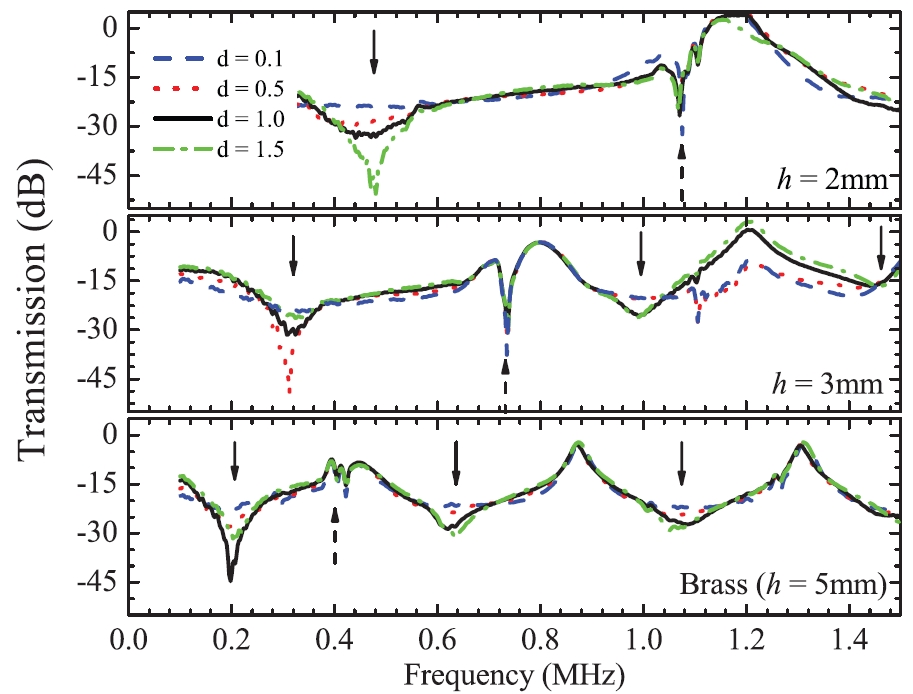
\includegraphics[width = 0.85\linewidth]{experimentRayleigh.jpg}
\caption{Experimental sound transmission spectra of a~water slit between two brass plates for different channel width $d$ and length $h$, reported in \cite{channel1}. The~vertical arrows indicate the~frequencies at which the~transmission is extraordinarily low. \textit{Image reprinted from \cite{channel1}, CC BY 3.0.}}
\label{fig:experimentRayleigh}
\end{center}
\end{figure}

Intuitively, the~reason for the~emergence of the~unexpected minima in \cref{fig:experimentRayleigh} has to be the~destructive interference of waves that propagate in the~channel --- the~same reason that explains the~Fabry-Perot resonances.
Of course, the~interfering waves must now be the~proper eigenmodes of the~system, that is, of the channel between the plates.
Further, I will present the~theory of sound transmission through a~slit formed by two solid plates, taking into account the~elastic nature of the~latter.
The~eigenmodes of the~system in question are essentially the~Rayleigh waves modified by coupling to the~fluid environment.
This modification makes the~eigenmodes lose their orthogonality with respect to each other.
Having a~nonorthogonal basis of eigenfunctions is quite typical for problems involving elastic solids, e.g., it is known that the~elastic modes of an~isolated solid plate (the~Rayleigh-Lamb modes) are not orthogonal as well \cite{achenbac}.
Moreover, the~channel eigenmodes belong to two main categories: the~true surface, or propagating, modes, and the~leaky modes, though the~nonorthogonality makes explicit separation of modes impossible.
The~latter observation applies also to electromagnetic domain, see, for example, discussion in \cite{sturman2} regarding the~metal-dielectric waveguides.

The~analytical solution to the~scattering problem relies on the~expansion of the~acoustic fields in series over both types of those coupled Rayleigh modes propagating in the~channel.
I also generalize the~approach to account for the~nonorthogonality of the~eigenmodes.
Ultimately, I will demonstrate how the~fluid channel that partially transmits sound via the~leaky waves effectively serves as a~redirecting acoustic antenna, and that the~effect of redirection of sound causes the~suppression of both transmission and reflection.
In the~rigid-body approximation, producing such an~effect is clearly infeasible.
For that reason, this effect should not be confused with other previously mentioned manifestations of the~strong suppression of sound \cite{norris4,estrada,estrada2,estrada3}, which introduce Fano-like resonances into the~transmission spectrum even in the~rigid-body approximation.
%The~complete basis of coupled Rayleigh eigenmodes will be used to expand the~acoustic fields in the~channel and the~plates in series.



%Here we develop a~theory of sound transmission through a~slit formed by two elastic solid plates. We solve the~eigenvalue problem for the~whole system which consists of two elastic infinite plates coupled through a~straight fluid channel. The~acoustic field is expanded over the~set of eigenfunctions which describe synchronized vibrations of the~whole system. Each eigenfunction is characterized by complex eigenvector, i.e. these eigenfunctions are {\it inhomogeneous} plane waves. Lack of orthogonality presents certain mathematical difficulties in calculations. Nevertheless, the~expansion over this nonorthogonal basis converges sufficiently fast, providing very good agreement with experimental results in the~whole frequency range.  Using the~proposed theory we show that at the~frequencies when the~deep minima in transmission are observed the~reflection  is also minimal.
%This occurs due to formation of quasi-standing Rayleigh wave in the~whole system.
%Since the~transmission and reflection are strongly suppressed, the~only way for the~accumulated elastic energy to escape is radiation into metal. 

%The~rate of radiation into metal is relatively  high, i.e. a~straight fluid channel serves as redirecting acoustic antenna. The~proposed mechanism is very different from the~ strong suppression of sound transmission through a~periodic arrangements of holes in a~rigid screen \cite{norris4,estrada,estrada2}. The~latter is due to destructive interference between the~Fabry-Perot cavity mode and the~Fourier component of the~acoustic field in the~fluid with the~wavelength equal to the~period of perforation.  This Fano-like resonance exists even in the~rigid-body approximation and is manifested as total reflection of sound wave from the~perforated solid plate. Unlike this, the~proposed effect of redirection of sound leads to suppression of both, transmission and reflection, and it vanishes in the~rigid-body approximation.


%%%%%%%%%%%%%%%%%%%%%%%%%%%%%%%%%%%%%%%%%%%%%%%%%%%%%%%%%%%%%%%%%%%%
\section{Acoustic Potentials}

\subsection{Scalar Potential for Pressure Waves in Fluids}

In this chapter, I neglect the~effects of viscosity and treat the~propagation of sound as a~laminar (nonturbulent) process in the~fluid which is otherwise stationary.
With that, only longitudinal pressure waves can exist within the~volume of the~fluid, and the~resulting pressure oscillations are known to be adiabatic, meaning that the~wave does not lose or gain energy from the~background.

The~complete description of the~fluid dynamics requires knowledge of either the~local velocity $\mathbf{v}_f(\mathbf{r}, t)$ or both the local pressure $p_f(\mathbf{r}, t)$ and density $\rho_f(\mathbf{r}, t)$ at any given position $\mathbf{r}$ and moment of time $t$.
These quantities are related since one must satisfy both the~continuity equation
\begin{equation}
\label{eq:continuityRayleigh}
\frac{\partial\rho_f}{\partial t} + \nabla\cdot\left(\rho_f\mathbf{v}_f\right) = 0,
\end{equation}
which guarantees the~conservation of mass in the~system, and the~momentum equation
\begin{equation}
\label{eq:secondNLRayleigh}
\frac{\partial \rho_f\mathbf{v}_f}{\partial t} + \nabla p_f = 0,
\end{equation}
which is essentially the~Newton's second law applied to a~unit volume of fluid.

Assuming the~propagating wave is only a~small perturbation of the~fluid stationary state, the~dynamic properties of the~fluid are linearized as
\begin{align}
p_f(\mathbf{r}, t)~&=~p_0 + p(\mathbf{r}, t), \label{eq:pressureLinearRayleigh}\\
\rho_f(\mathbf{r}, t)~&=~\rho_0 + \rho(\mathbf{r}, t), \label{eq:densityLinearRayleigh}\\
\mathbf{v}_f(\mathbf{r}, t)~&=~\mathbf{v}_0 + \mathbf{v}(\mathbf{r}, t), \label{eq:velocityLinearRayleigh}
\end{align}
where $p_0$, $\rho_0$, and $\mathbf{v}_0$ describe the~background acoustic field, and the~smallness of perturbations can be understood, for example, as $|p(\mathbf{r}, t)| \ll p_0$.
The~assumption of no background flow gives $\mathbf{v}_0=0$, and the~absence of the vortices yields $\nabla\times\mathbf{v}(\mathbf{r}, t)=0$.

The~longitudinal sound wave propagates with a~constant phase speed, which is given by
\begin{equation}
c_f = \sqrt{\left(\frac{\partial p_f}{\partial \rho_f}\right)_s},
\end{equation}
where the~derivative is calculated for an~adiabatic process, i.e., at constant entropy.
Using \cref{eq:pressureLinearRayleigh}-\cref{eq:densityLinearRayleigh}, one can relate the~local variations of pressure and density as
\begin{equation}
p(\mathbf{r}, t) = \rho(\mathbf{r}, t)c_f^2.
\end{equation}

Consequently, the~wave equation for the~pressure $p(\mathbf{r},t)$,
\begin{equation}
\label{eq:waveeqPRayleigh}
\Delta p - \frac{1}{c_f^2}\frac{\partial^2 p}{\partial t^2}~=~0,
\end{equation}
is immediately obtained after one substitutes \cref{eq:secondNLRayleigh} into \cref{eq:continuityRayleigh} and uses the~linearizations \cref{eq:pressureLinearRayleigh}-\cref{eq:velocityLinearRayleigh} while discarding the~terms that are quadratic over small perturbation.
%
The~condition $\nabla\times\mathbf{v}(\mathbf{r}, t) = 0$ allows to represent the~velocity as a~gradient of a~scalar function (fluid is then said to be in a state of a potential flow):
\begin{equation}
\mathbf{v}(\mathbf{r}, t)=\nabla B(\mathbf{r}, t).
\end{equation}
For monochromatic waves with the~time dependence given by $e^{-i\omega t}$ factor, the~equation \cref{eq:secondNLRayleigh} relates the~velocity to the~gradient of pressure
\begin{equation}
\label{eq:vandpRayleigh}
i\omega\rho_0\mathbf{v}(\mathbf{r},t) = \nabla p(\mathbf{r},t),
\end{equation}
and, therefore, one may define the~acoustic potential $B(\mathbf{r}, t)$ as
\begin{equation}
\label{eq:potentialBRayleigh}
B(\mathbf{r}, t) = \frac{p(\mathbf{r},t)}{i\omega\rho_0}.
\end{equation}
From \cref{eq:waveeqPRayleigh}-\cref{eq:potentialBRayleigh} it is obvious that the~potential $B(\mathbf{r}, t)$ satisfies the~wave equation
\begin{equation}
\label{eq:waveeqBRayleigh}
\Delta B - \frac{1}{c_f^2}\frac{\partial^2 B}{\partial t^2}~=~0,
\end{equation}
and that it uniquely defines the~local pressure and velocity of the~fluid.

Since the~density variations are small, the~approximate equality $\rho_f(\mathbf{r}, t) \approx \rho_0$ holds, and in the~sections below I will not distinguish between these two quantities and will use the~notation $\rho_f$ instead of $\rho_0$.


\subsection{Scalar and Vector Potentials for Elastic Waves in Solids}

Unlike fluids which take the~shape of the~volume they occupy, the~elastic properties of solids allow them to resist the~changes to their shape in order to reestablish their original form and size.
As a~result, two distinct types of waves can propagate in the~bulk of a~solid --- longitudinal (compressional) and transverse (shear).
In these waves, the~particle oscillations occur either along or perpendicular to the~direction of wave propagation, respectively.
The~local displacement field $\mathbf{u}(\mathbf{r},t)$ and stress tensor $\sigma_{ik}(\mathbf{r}, t)$ are typically used to describe the~dynamics of a~solid.
The~Newton's second law applied to a~unit volume of the~solid
\begin{equation}
\rho_m\frac{\partial u_i}{\partial t} = \frac{\partial \sigma_{ik}}{\partial x_k},
\end{equation}
where the~Einstein summation convention for tensors is implied, ultimately leads to the~following general wave equation for elastic waves \cite{LLtom7}:
\begin{equation}
\label{eq:waveeqURayleigh}
\frac{\partial^2 \mathbf{u}}{\partial t^2}~=~c_t^2 \Delta\mathbf{u} + \left(c_l^2-c_t^2\right)\nabla\left(\nabla\cdot\mathbf{u}\right).
\end{equation}
Here $\rho_m$ is the~density of the~solid and $c_l$($c_t$) is the~speed of the~pure longitudinal (transverse) acoustic wave.
The~two speeds of sound are expressed through the~so-called Lam\'e parameters of the~solid, $\lambda$ and $\mu$:
\begin{equation}
c_l~=~\sqrt{\frac{\lambda+2\mu}{\rho}}, \qquad c_t~=~\sqrt{\frac{\mu}{\rho}},
\end{equation}
which in their turn represent the~bulk and shear moduli $K$ and $G$:
\begin{equation}
K~=~\lambda+\frac23\,\mu, \qquad G~=~\mu.
\end{equation}

Since, according to the~Helmholtz decomposition theorem, the~vector quantity $\mathbf{u}(\mathbf{r},t)$ can always be represented as a~sum of a~potential and a~solenoidal field:
\begin{equation}
\mathbf{u} = \mathbf{u}_l + \mathbf{u}_t,
\end{equation}
where $\nabla\times\mathbf{u}_l = 0$ and $\nabla\cdot\mathbf{u}_t = 0$, it allows splitting \cref{eq:waveeqURayleigh} into two independent wave equations
\begin{equation}
\label{eq:waveeqUltRayleigh}
\Delta\mathbf{u}_{l,t} - \frac{1}{c_{l,t}^2}\frac{\partial^2 \mathbf{u}_{l,t}}{\partial t^2}~=~0
\end{equation}
for both longitudinal and transverse components of the~elastic wave and introduce the~scalar potential $L(\mathbf{r}, t)$ and the~vector potential $\mathbf{S}(\mathbf{r}, t)$ as
\begin{equation}
\mathbf{u}_l(\mathbf{r}, t)~=~\nabla L(\mathbf{r}, t), \qquad \mathbf{u}_t(\mathbf{r}, t)~=~\nabla\times\mathbf{S}(\mathbf{r}, t).
\end{equation}

With the~scalar potential $L$ corresponding to the~pressure wave and the~vector potential $\mathbf{S}$ representing the~shear wave, naturally, they satisfy the~respective wave equations:
\begin{align}
\Delta L - \frac{1}{c_l^2}\frac{\partial^2 L}{\partial t^2}~&=~0, \label{eq:waveeqLRayleigh}\\
\Delta \mathbf{S} - \frac{1}{c_t^2}\frac{\partial^2 \mathbf{S}}{\partial t^2}~&=~0, \label{eq:waveeqSRayleigh}
\end{align}
and uniquely define the~local displacement of the~solid
\begin{equation}
\label{eq:displacementRayleigh}
\mathbf{u}(\mathbf{r}, t)~=~\nabla L(\mathbf{r}, t) + \nabla\times\mathbf{S}(\mathbf{r}, t)
\end{equation}
and stress tensor (through Hooke's law)
\begin{equation}
\label{eq:HookesLawRayleigh}
\sigma_{ik}(\mathbf{r}, t)~=~\lambda u_{ll}(\mathbf{r}, t)\delta_{ik} + 2\mu u_{ik}(\mathbf{r}, t).
\end{equation}
Here $u_{ik}$ denotes the~strain tensor $u_{ik}=\frac12\left(\frac{\partial u_i}{\partial x_k}+\frac{\partial u_k}{\partial x_i}\right)$, and $\delta_{ik}$ is the~Kronecker delta.

Note that the~potentials themselves are not defined uniquely, specifically, adding a~curl of an~arbitrary vector function to $L(\mathbf{r}, t)$ or adding a~gradient of an~arbitrary scalar function to $\mathbf{S}(\mathbf{r}, t)$ does not change the~displacement field $\mathbf{u}(\mathbf{r}, t)$.


\subsection{Fluid-Solid Boundary Conditions}

When a~fluid and a~solid occupy adjacent regions of space, the~boundary conditions must be specified at the~fluid-solid interface (see \cite{lloyd}, for example).
The~continuity of the~normal component of the~local velocity
\begin{equation}
\label{eq:boundaryVelocityRayleigh}
\left.v_n\right|_\Sigma~=~\left.\dot{u}_n\right|_\Sigma
\end{equation}
ensures that the~two media neither permeate each other nor produce void regions between them along the~interface $\Sigma$.
As the~fluid is nonviscous, there is no binding between the~tangential components of velocities, and the~particles of the~fluid do not stick to the~surface of the~solid.

Other than that, the~balance between the~stress of the solid and the~pressure in the~fluid
\begin{equation}
\label{eq:boundaryStressRayleigh}
\left.\sigma_{ik}n_k\right|_\Sigma = - \left.p n_i\right|_\Sigma
\end{equation}
must be enforced.
Here the~vector $n_i$ is the~external normal to the~surface $\Sigma$, and due to the~absence of shear interactions in fluid its pressure is acting perpendicular to $\Sigma$: $p_i = -p n_i$.



%%%%%%%%%%%%%%%%%%%%%%%%%%%%%%%%%%%%%%%%%%%%%%%%%%%%%%%%%%%%%%%%%%%%
\section{Rayleigh Waves on the~Surface of a~Solid}

When considering the~propagation of elastic waves in the~bulk of a~solid, one infers the~independence of pressure waves from shear waves in the~sense that the~wave amplitudes are not tied to each other.
However, a~specific relationship between the~amplitudes arises when the~waves propagate close to the~surface of the~solid, which requires satisfying the~boundary conditions \cref{eq:boundaryVelocityRayleigh}-\cref{eq:boundaryStressRayleigh}.
In particular, the~wave equation \cref{eq:waveeqURayleigh} was shown to have a~surface wave solution --- the~so-called Rayleigh wave \cite{rayleigh}, which intertwines both longitudinal and transverse particle motion and is concentrated in the~vicinity of the~surface, exponentially vanishing away from it.
The~Rayleigh waves are typically distinguished from the~Lamb waves, which are the~elastic surface waves as well, but are specific for the~thin solid plates.

%\subsection{Solid-Vacuum Interface}

The~concept of Rayleigh waves is normally demonstrated in the~simplified situation, where the~solid borders with the~vacuum \cite{LLtom7}.
Here I assume the~planar interface that coincides with the~plane $z=0$ (where the~region $z>0$ is occupied by solid), and I seek the~monochromatic solution to \cref{eq:waveeqLRayleigh}-\cref{eq:waveeqSRayleigh} which propagates in the~$x$-direction and exponentially decays with $z$.
This solution is only valid in the~region $z\ge 0$, as in the~vacuum the~sound does not propagate.

The~independent of the~coordinate $y$ acoustic potentials can thus be written down as
\begin{align}
L(x,z,t)~&=~l\,e^{i\beta x-\nu z-i\omega t}, \qquad z \ge 0, \\
\mathbf{S}(x,z,t)~&=~\mathbf{s}\,e^{i\beta x-\eta z-i\omega t}, \qquad z \ge 0,
\end{align}
where $\beta$ is the~$x$-component of the~wavevector, $l$ and $\mathbf{s} = (s_x, s_y, s_z)$ are the~amplitudes of the~potentials.
The~quantities $\nu$ and $\eta$ are defined as
\begin{align}
\nu~&=~\sqrt{\beta^2-k_l^2}, &\beta \ge k_l=\frac{\omega}{c_l}, \label{eq:nuRayleigh}\\
\eta~&=~\sqrt{\beta^2-k_t^2}, &\beta \ge k_t=\frac{\omega}{c_t}. \label{eq:etaRayleigh}
\end{align}
%
The~components of the~displacement field are calculated from the~potentials using \cref{eq:displacementRayleigh}:
\begin{align}
u_x~&=~\frac{\partial L}{\partial x} - \frac{\partial S_y}{\partial z}~=~\left(i\beta e^{-\nu z}\cdot l+\eta e^{-\eta z}\cdot s_y\right)e^{i\beta x-i\omega t}, \label{eq:uxRayleigh}\\
u_y~&=~\frac{\partial S_x}{\partial z} - \frac{\partial S_z}{\partial x}~=~-\left(\eta\cdot s_x+i\beta \cdot s_z\right)e^{-\eta z}e^{i\beta x-i\omega t}, \label{eq:uyRayleigh}\\
u_z~&=~\frac{\partial L}{\partial z} + \frac{\partial S_y}{\partial x}~=~\left(-\nu e^{-\nu z}\cdot l+i\beta e^{-\eta z}\cdot s_y\right)e^{i\beta x-i\omega t}. \label{eq:uzRayleigh}
\end{align}

The~solid-vacuum boundary is a~free boundary, so one may only demand that any infinitesimal part of the~interface is stress-free, namely, that
\begin{equation}
\sigma_{xz}~=~\sigma_{yz}~=~\sigma_{zz}~=~0,
\end{equation}
at the~interface $z=0$, or, more explicitly,
\begin{equation}
\label{eq:sigmaxzyzzzRayleigh}
\left\{\begin{array}{rll}
0~=~\sigma_{xz}~&=~2\mu u_{xz}~&=~\mu \left(\dfrac{\partial u_x}{\partial z}+\dfrac{\partial u_z}{\partial x}\right), \\
0~=~\sigma_{yz}~&=~2\mu u_{yz}~&=~\mu \dfrac{\partial u_y}{\partial z}, \\
0~=~\sigma_{zz}~&=~2\mu u_{zz}+\lambda \nabla\cdot\mathbf{u}~&=~2\mu \dfrac{\partial u_z}{\partial z} + \lambda\left(\dfrac{\partial u_x}{\partial x}+\dfrac{\partial u_z}{\partial z}\right).
\end{array}\right.
\end{equation}

The~second equation in the~system suggests that $u_y = 0$, and without any loss of generality one may equate both $s_x$ and $s_z$ to zero, thus leaving $s_y$ as the~only nonzero component of the~coefficient $\mathbf{s}$.
This becomes possible due to the~fact that one may add a~gradient of any scalar function to $\mathbf{S}(\mathbf{r}, t)$ without any effect on the~displacement field.
If one now selects this scalar function to be $f(\mathbf{r}, t) = \left(s_z/\eta\right) e^{i\beta x-\eta z-\i\omega t}$, then the~redefined potential $\mathbf{S}'(\mathbf{r}, t) = \mathbf{S}(\mathbf{r}, t) + \nabla f(\mathbf{r}, t)$ will automatically have $S'_z = 0$, and it will also have $S'_x = 0$ due to the~relation \cref{eq:uyRayleigh} and the~condition $u_y=0$.
With this, I will further assume the~vector potential to have only nonzero $y$-component, $\mathbf{S}(\mathbf{r}, t) = \left(0, S(\mathbf{r}, t), 0\right)$, and $\mathbf{s}=\left(0,s,0\right)$.
It is worth mentioning that even though the~wave is propagating along the~$x$-axis, its amplitude, nevertheless, varies with the~coordinate $z$, causing the~vector potential to give a~nonzero contribution to the~displacement $u_x$, and it is thus impossible to break down the~Rayleigh wave into independent longitudinal and transverse components.

Now, using \cref{eq:uxRayleigh}-\cref{eq:uzRayleigh}, the~first and the~third equations from \cref{eq:sigmaxzyzzzRayleigh} are reduced to
\begin{equation}
\left\{\begin{array}{rrrr}
\left(\beta^2+\eta^2\right)\cdot s &+&2i\beta\nu\cdot l~&=~0, \\
-2i\mu\beta\eta\cdot s &+& \left(2\mu\nu^2-\lambda k_l^2\right)\cdot l~&=~0, \\
\end{array}\right.
\end{equation}
The~obtained system has a~nontrivial solution if and only if its determinant equals zero, namely, if
\begin{equation}
\frac{1}{\mu}\left(2\mu\nu^2-\lambda k_l^2\right)\left(\beta^2+\eta^2\right)-4\beta^2\eta\nu~=~0,
\end{equation}
or, when simplified,
\begin{equation}
\left(\eta^2+\beta^2\right)^2-4\nu\eta\beta^2~=~0.
\end{equation}

The~latter expression implicitly relates the~frequency of the~wave $\omega$ and its wavevector $\beta$, and it can be rewritten for the~dimensionless phase velocity $\xi=\omega/\beta c_t$ as
\begin{equation}
\label{eq:dispNoRHSRayleigh}
\left(2-\xi^2\right)^2-4\sqrt{1-\xi^2}\sqrt{1-\frac{c_t^2}{c_l^2}\xi^2}~=~0.
\end{equation}
Since typically $c_t < c_l$ in solids, the~equation \cref{eq:dispNoRHSRayleigh} has only one real root for any value of $c_t/c_l$ which lies in the~range $0 < \xi < 1$; for most common solids, the~dimensionless phase speed is restricted to the~range $0.874 \le \xi \le 0.955$ \cite{LLtom7}.
Such values of $\xi$ describe surface waves which propagate slower than either the~pure pressure or shear wave in the~bulk of the~solid.
For any given solid, the~speed of the~Rayleigh wave is uniquely defined by the~ratio of its transverse and longitudinal speeds of sound, and does not depend on the~wave frequency.

%\subsection{Solid-Fluid Interface}


%%%%%%%%%%%%%%%%%%%%%%%%%%%%%%%%%%%%%%%%%%%%%%%%%%%%%%%%%%%%%%%%%%%%
\section{Coupled Rayleigh Waves in the~Fluid Channel between Two Solid Plates}

\begin{figure}
\begin{center}
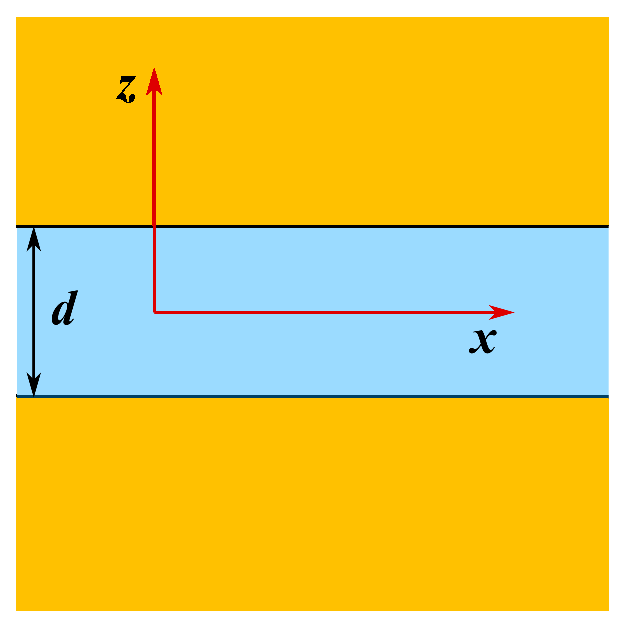
\includegraphics[width=0.5\linewidth]{infinite.eps}
\caption{An~infinite fluid channel between two elastic plates.}
\label{fig:infinite}
\end{center}
\end{figure}

Now I consider a~monochromatic sound wave propagating along an~infinite straight fluid channel of the~width $d$ between two elastic plates (see \cref{fig:infinite}).
The~elastic plates are made from the~same material and they are occupying the~regions $|z| > d/2$.
The~wave is propagating in the~positive $x$-direction.
The~mirror symmetry with respect to the~$xOy$ plane suggests that the~eigenmodes of the~system are either even or odd functions of the~coordinate $z$.
More precisely, I will be using the~term "even" to describe the~eigenmodes with $u_x$ being an~even and $u_z$ being an~odd function of $z$.
The~term "odd" will then refer to any mode with $u_x$ being an~odd function of $z$.
In terms of potentials, the~even mode corresponds to all potentials being even functions of $z$.

Below, I will analyze only the~even modes and pay no attention to the~odd modes.
The~reason for that is the~mirror symmetry with respect to the~$x$-axis that will be enforced everywhere in the~subsequent sections.
For the~scattering problem it means that the~impinging wave should be incident only normally at the~system, along the~$x$-axis.
The~excitation of the~odd modes will not be possible at all as they violate the~symmetry.
However, the~odd modes can be excited if the~problem loses its symmetry with respect to $xOy$ plane, either by allowing the~oblique incidence of the~sound wave or by having the~elastic plates made from different materials \cite{channel1}.

\subsection{Dispersion Relation}

The~symmetric solution of the~wave equations \cref{eq:waveeqBRayleigh}, \cref{eq:waveeqLRayleigh}, and \cref{eq:waveeqSRayleigh} is as follows (the~factor $e^{-i\omega t}$ is omitted everywhere below):
\begin{align}
B(x,z)~&=~b\,e^{i\beta x}\cos{kz}, &|z| < d/2, \label{eq:potBcoupledRayleigh}\\
L(x,z)~&=~l\,e^{i\beta x-\nu|z|}, &|z| > d/2, \label{eq:potLcoupledRayleigh}\\
S_y(x,z)~&=~s\,e^{i\beta x-\eta|z|}, \qquad S_x=S_z=0, &|z| > d/2, \label{eq:potScoupledRayleigh}
\end{align}
where $k=\sqrt{k_f^2-\beta^2}$, $k_f=\omega/c_f$.
Both $\nu$ and $\beta$ are defined as earlier in \cref{eq:nuRayleigh}-\cref{eq:etaRayleigh} except that no restriction is placed on the~value of $\beta$.

Because of the~symmetry, it is sufficient to write the~boundary conditions only for, e.g. $z=d/2$.
At this fluid-metal interface the~stress and the~normal component of the~velocity are continuous:
\begin{equation}
\sigma_{zz}~=~-p, \qquad \sigma_{xz}~=~0, \qquad \dot{u}_z~=~v_z,
\end{equation}
as follows from \cref{eq:boundaryVelocityRayleigh}-\cref{eq:boundaryStressRayleigh}.
The~stress tensor component $\sigma_{yz}$ is identically zero due to the~choice of the~vector potential $\mathbf{S}$.

Similarly to the~derivations in the~previous section, the~boundary conditions yield the~following system where all the~potentials are evaluated at $z=d/2$:
\begin{equation}
\left\{\begin{aligned}
-\lambda k_l^2 L +2\mu\left(\frac{\partial^2 L}{\partial z^2}+\frac{\partial^2 S}{\partial x \partial z}\right)~&=~-i\omega\rho_f B, \\
\mu\left(2\frac{\partial^2 L}{\partial x \partial z}+\frac{\partial^2 S}{\partial x^2}-\frac{\partial^2 S}{\partial z^2}\right)~&=~0, \\
-i\omega\left(\frac{\partial L}{\partial z} + \frac{\partial S_y}{\partial x}\right)~&=~\frac{\partial B}{\partial z},
\end{aligned}\right.
\end{equation}
which is reduced to
\begin{equation}
\label{eq:coeffRelationsRayleigh}
\left\{
\begin{array}{rrrrrr}
\left(2\mu\nu^2-\lambda k_l^2\right)\,e^{-\nu d/2}\cdot l &-& 2i\mu \eta \beta\,e^{-\eta d/2}\cdot s &+& i\omega\rho_f \cos(k d/2)\cdot b~&=~0, \\
2i\nu \beta \,e^{-\nu d/2}\cdot l &+& \left(\beta^2 +\eta^2 \right)e^{-\eta d/2} \cdot s &&~&=~0, \\
i\omega\nu \,e^{-\nu d/2}\cdot l &+& \omega\beta \,e^{-\eta d/2}\cdot s &+& k \sin(k d/2)\cdot b~&=~0. \\
\end{array}
\right.
\end{equation}
This set of homogeneous linear equations has a~nontrivial solution if its determinant vanishes, which is expressed by the~condition
\begin{equation}
\label{eq:dispersionkRayleigh}
\left(\eta^2+\beta^2\right)^2-4\nu\eta\beta^2~=~\frac{\rho_f}{\rho_m}\frac{\omega^4}{c_t^4}\frac{\nu}{k}\,\cot \frac{kd}{2}.
\end{equation}
Since all the~quantities $k$, $\nu$, and $\eta$ are expressed through $\omega$ and $\beta$, the~latter equation is essentially the~dispersion relation for the~coupled Rayleigh waves propagating in the~fluid channel.
This relation can be rewritten in terms of the~dimensionless frequency $\Omega = \omega d/c_t$ and wavevector $q = \beta d$, which allows to eliminate the~dependence on the~channel width $d$ from the~picture:
\begin{equation}
\label{eq:dispersionqRayleigh}
\left(2 q^2-\Omega^2\right)^2 - 4 q^2 \sqrt{q^2 - (c_t/c_l)^2 \Omega^2} \sqrt{q^2 - \Omega^2} 
~=~ \frac{\rho_f}{\rho_m}\Omega^4 \sqrt{\frac{q^2 - (c_t/c_l)^2 \Omega^2}{(c_t/c_f)^2 \Omega^2 - q^2}}\,\cot\left( \frac{1}{2}\sqrt{\frac{c_t^2}{c_f^2} \Omega^2 - q^2}\right).
\end{equation}
Also, the~dispersion relation for the~dimensionless phase velocity $\xi=\omega/\beta c_t$ can be obtained from the~latter by substituting $q=\Omega /\xi$:
\begin{equation}
\label{eq:dispersionXiRayleigh}
\left(2-\xi^2\right)^2-4\sqrt{1-\xi^2}\sqrt{1-\frac{c_t^2}{c_l^2}\xi^2}
~=~\frac{\rho_f}{\rho_m}\,\xi^4 \sqrt{\frac{1-\left(c_t/c_l\right)^2\xi^2}{\left(c_t/c_f\right)^2\xi^2-1}}\cot\!\left(\frac{\Omega}{2\xi}\sqrt{\frac{c_t^2}{c_f^2} \xi^2-1}\,\right).
\end{equation}
Real and complex solutions of the~dispersion relation \cref{eq:dispersionqRayleigh} define the~allowed values of the~wave vector $q = q(\Omega)$ for each frequency $\Omega$, and \cref{eq:dispersionXiRayleigh} gives the~allowed phase velocities $\xi = \xi(\Omega)$.


\subsection{Analysis of the~Dispersion Branches}

For any frequency $\Omega$, the~dispersion equation \cref{eq:dispersionXiRayleigh} has a~finite number of real ($\xi = \re \xi > 0$) and an~infinite number of complex ($\re \xi > 0$, $\im \xi < 0$) roots.
The~condition $\re\xi>0$ ensures that the~eigenmodes found indeed propagate forward in the~$+x$-direction.
Since the~phase speed $\xi$ enters \cref{eq:dispersionXiRayleigh} only as $\xi^2$, it is obvious that a~negative of any root $\xi$ with a~positive real part also satisfies the~dispersion equation.
Such roots describe the~backward propagating Rayleigh waves, i.e., in the~$-x$-direction.

In the~numerical analysis below, I will be using the~parameters of water ($\rho_f=1000$ kg/m$^3$, $c_f=1500$ m/s) and brass ($\rho_m=8400$ kg/m$^3$, $c_t=2000$ m/s, $c_l=4250$ m/s).

\subsection{Real Eigenmodes}

The~eigenmodes with real $\xi$ have real wavevector $q$, and, therefore, they are propagating modes.
If the~losses in the~media are neglected, these true modes will never decay as they propagate along the~channel.
Due to the~term $\sqrt{1-\xi^2}$ in \cref{eq:dispersionXiRayleigh}, the~value of $\xi$ must be restricted to the~range $0 < \xi \le 1$.
This means that in \cref{eq:potBcoupledRayleigh}-\cref{eq:potScoupledRayleigh} the~values of $\beta$, $\nu$, and $\eta$ are purely real which provides the~oscillating behavior along the~channel and the~decay of the~acoustic field into the~solid away from the~channel.
As for the~value of $k$, it may be either purely real (when $c_f/c_t < \xi \le 1$) or purely imaginary (when $0 < \xi < c_f/c_t$).
Here I assume that $c_f < c_{l,t}$, since the~speed of sound in fluids is considerably lower than the~speed of sound in solids.
%
In the~first case, the~acoustic potential in the~fluid oscillates along $z$ as well and the~sound wave has a~wavefront of constant amplitude inside the~channel.
The~two Rayleigh waves on each fluid-solid interface are strongly coupled as the~sound energy is not concentrated in the~vicinity of either interface but rather confined to the~whole width of the~channel.
In the~second case, the~potential \cref{eq:potBcoupledRayleigh} becomes $B(x,z)=b\,e^{ibx}\cos{kz}=b\,e^{ibx}\cosh{|kz|}$, so that the~sound energy both in the~solid and in the~fluid is mostly concentrated near the~interfaces. 

These two types of true eigenmodes will further be referred to as fast and slow modes since the~former propagate faster than the~speed of sound in fluid, and the~latter propagate slower, respectively.

The~dispersion equation \cref{eq:dispersionXiRayleigh} is transcendental and can only be solved numerically.
Nevertheless, a~certain asymptotic analysis of the~eigenmode dispersion is still possible.
I start by considering the~fast modes.
I note that the~left-hand side of \cref{eq:dispersionXiRayleigh} is clearly identical to that of \cref{eq:dispNoRHSRayleigh}.
Its right-hand side thus describes the~coupling of two individual Rayleigh waves on each interface through the~fluid.
The~coupling strength is proportional to the~ratio $\rho_f/\rho_m$. 
In the~absence of the~fluid, $\rho_f=0$, the~coupling term disappears and the~surface waves in each plate become uncoupled.
These surface waves are the~same Rayleigh waves described by \cref{eq:dispNoRHSRayleigh}, with their phase speed $\xi=\xi_R$ independent from the~frequency.
Thus in the~limit $\rho_f/\rho_m \ll 1$, when the~right-hand side of \cref{eq:dispersionXiRayleigh} is small, the~coupled Rayleigh waves should be almost dispersionless.

However, the~previous argument cannot be valid if the~argument of the~cotangent $kd/2$ is close to an~integer of $\pi$, in which case the~value of the~cotangent outmatches the~smallness of $\rho_f/\rho_m$.
The~condition $kd/2\pi=0,1,2,...$ corresponds to the~potential \cref{eq:potBcoupledRayleigh} being a~standing wave with its velocity nodes at the~channel walls, which can be seen by calculating $v_z$:
\begin{equation}
\left.v_z(x,z)\right|_{z=\frac{d}{2}}~=~\left.\frac{\partial B}{\partial z}\right|_{z=\frac{d}{2}}~=~-kb e^{i\beta x}\sin{\frac{kd}{2}}~=~0.
\end{equation}
In other words, the~coupled Rayleigh wave behaves identically to a~waveguide mode of a~channel with ideally rigid walls.
The~dispersion of the~symmetric waveguide modes consists of an~infinite number of branches
\begin{equation}
\label{eq:waveguideRayleigh}
\omega_n=c_f\sqrt{\left(\frac{2\pi n}{d}\right)^2+\beta^2}, \qquad n=0,1,2,...
\end{equation}
These branches serve as asymptotic boundaries for the~dispersion branches of the~coupled Rayleigh waves.
Each waveguide mode appears after its respective cutoff frequency with the~wavevector $\beta=0$, and features an~infinite phase velocity $\omega_n/\beta$ (except for the~mode $n=0$).

Similar to the~waveguide modes, each individual Rayleigh modes also emerges only after a~corresponding cutoff frequency.
However, the~condition $\beta=0$ does not define the~cutoff frequency in this case since the~phase speed $\xi$ of the~fast modes cannot be infinite: $c_f/c_t < \xi \le 1$.
Clearly, every new dispersion branch must then start with $\xi=1$, which gives the~dimensionless cutoff frequencies
\begin{equation}
\label{eq:cutoffRayleigh}
\Omega_{n} = \frac{\omega_n d}{c_t}= \frac{2}{\sqrt{(c_t/c_f)^2 -1}} \left[ \pi \left(n-1\right) +
\arctan\left(\frac{\rho_f}{\rho_m} \sqrt{\frac{1-(c_t/c_l)^2}{(c_t/c_f)^2-1}}\, \right)\right] ,\,\, n = 1,2, \dots
\end{equation}
and the~corresponding dimensionless wavevectors $q_n = \Omega_n/\xi = \Omega_n$.

Even for the~first fast mode the~cutoff frequency $\Omega_1$ is nonzero, and thus in the~limit of low frequencies no fast modes can be excited to propagate in the~fluid channel.

Unlike the~fast modes, the~single slow coupled Rayleigh mode exists in the~whole frequency range starting from $\Omega=0$ with $\xi=0$ and asymptotically approaching $\xi=c_f/c_t$ when $\Omega \rightarrow \infty$.
The~slow mode is characterized by purely imaginary $k$, and its dispersion equation
\begin{equation}
\label{eq:dispSlowRayleigh}
\left(2-\xi^2\right)^2-4\sqrt{1-\xi^2}\sqrt{1-\frac{c_t^2}{c_l^2}\xi^2}
~=~-\frac{\rho_f}{\rho_m}\,\xi^4 \sqrt{\frac{1-\left(c_t/c_l\right)^2\xi^2}{1-\left(c_t/c_f\right)^2\xi^2}}\coth\!\left(\frac{\Omega}{2\xi}\sqrt{1-\frac{c_t^2}{c_f^2} \xi^2}\,\right)
\end{equation}
is derived using \cref{eq:potBcoupledRayleigh}-\cref{eq:dispersionkRayleigh}, where $k=i|k|$ and $\cos kz$ is replaced with $\cosh |kz|$ in the~expression for the~potential $B(x,z)$.

For $\xi \ll 1$ and $\Omega \ll 1$, I expand the~left-hand side of the~latter dispersion equation in series over $\xi$ and keep the~most significant term only:
\begin{equation}
-2\left(1-\frac{c_t^2}{c_l^2}\right)\xi^2~\approx~-\frac{\rho_f}{\rho_m}\xi^4 \coth \frac{\Omega}{2\xi}.
\end{equation}
Under the~additional assumption $\Omega \ll \xi$ (which is justified by solving the~dispersion equation at low frequencies numerically) the~cotangent $\coth\dfrac{\Omega}{2\xi}$ can be replaced by its approximate value $\dfrac{2\xi}{\Omega}$, and one obtains
\begin{equation}
\xi^3~\approx~\frac{\rho_m}{\rho_f}\left(1-\frac{c_t^2}{c_l^2}\right)\Omega
\end{equation}
or, in terms of the~wavevector $q=\Omega/\xi$,
\begin{equation}
\label{eq:asymptSlowRayleigh}
\Omega~\approx~\sqrt{\frac{\rho_m}{\rho_f}\left(1-\frac{c_t^2}{c_l^2}\right)}\,q^{3/2}.
\end{equation}
It appears that the~slow mode exhibits an~essentially nonlinear dispersion in the~long-wavelength limit, with the~vanishing phase and group velocities for $\Omega=0$.
The~low-frequency waveguide mode \cref{eq:waveguideRayleigh}, however, features purely linear dispersion (for $n=0$).
This means that the~subwavelength propagation of sound through a~fluid channel is drastically different for the~cases of a~real channel with vibrating walls and of an~ideal channel with rigid walls.
The~same is known for the~transmission of electromagnetic waves through a~deeply subwavelength metallic slit, in which case some interesting features arise that do not exist for perfectly conducting screens \cite{seo,xia}.

In the~high-frequency limit the~phase speed of the~slow mode is bound by the~condition $\xi < c_f/c_t$.
More precisely, the~phase speed $\xi$ asymptotically approaches a~specific value $\xi_{a}$: $\xi \rightarrow \xi_{a} < c_f/c_t$.
This limiting phase speed $\xi_a$ satisfies the~equation
\begin{equation}
\left(2-\xi_a^2\right)^2-4\sqrt{1-\xi_a^2}\sqrt{1-\frac{c_t^2}{c_l^2}\xi_a^2}
~=~-\frac{\rho_f}{\rho_m}\,\xi_a^4 \sqrt{\frac{1-\left(c_t/c_l\right)^2\xi_a^2}{1-\left(c_t/c_f\right)^2\xi_a^2}},
\end{equation}
which is obtained from \cref{eq:dispSlowRayleigh} for high frequencies $\Omega$, where the~value of hyperbolic cotangent is approximately $1$ for large arguments.
The~deviation of $\xi_a$ from $c_f/c_t$ is small whenever the~ratio $\rho_f/\rho_m$ is small.
To demonstrate this, I rearrange the~latter equation as
\begin{equation}
\sqrt{c_f/c_t-\xi_a}\sqrt{c_f/c_t+\xi_a}~=~\frac{\rho_f}{\rho_m}\frac{\left(c_f/c_t\right)\xi_a^4 \sqrt{1-\left(c_t/c_l\right)^2\xi_a^2}}{4\sqrt{1-\xi_a^2}\sqrt{1-\left(c_t/c_l\right)^2\xi_a^2}-\left(2-\xi_a^2\right)^2},
\end{equation}
and for $\rho_f/\rho_m \ll 1$ the~value of $\xi_a$ can be replaced by $c_f/c_t$ everywhere except under the~first square root in the~left-hand side.
This yields
\begin{equation}
\label{eq:xiaRayleigh}
\frac{c_f}{c_t}-\xi_a \approx \frac12\left(\frac{\rho_f}{\rho_m}\right)^2 \left(\frac{\left(c_f/c_t\right)^{9/2} \sqrt{1-\left(c_f/c_l\right)^2}}{4\sqrt{1-\left(c_f/c_t\right)^2}\sqrt{1-\left(c_f/c_l\right)^2}-\left(2-\left(c_f/c_t\right)^2\right)^2}\right)^2.
\end{equation}
The~phase speed of the~slow mode then has the~following asymptotic dependence on the~frequency:
\begin{equation}
\left(\xi_a-\xi\right) \sim e^{-\Omega}, \qquad \Omega \rightarrow \infty,
\end{equation}
which originates from the~approximation $\coth \left(\Omega/2\right) \approx 1+2e^{-\Omega}$ for large values of $\Omega$.
The~dispersion of the~slow mode is then almost linear, $\Omega \approx \xi_a q$, and the~mode propagates slightly slower than the~pure pressure wave in the~fluid.


\begin{figure}
\begin{center}
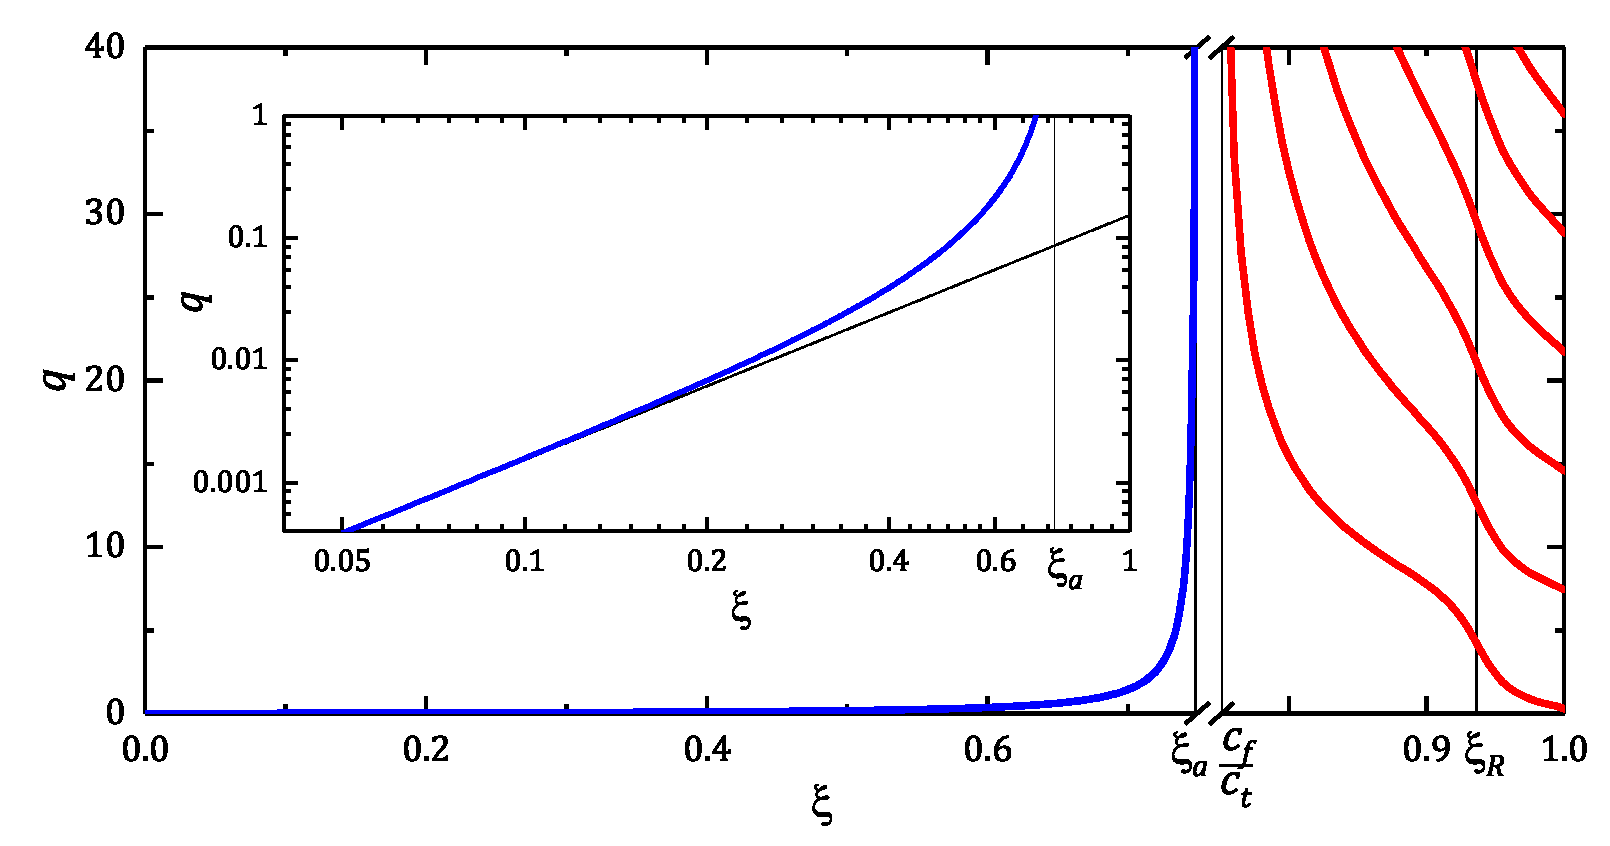
\includegraphics[width=\linewidth]{xi-q.eps}
\caption{Dimensionless phase velocity $\xi=\Omega/q$ vs wave vector $q=\beta d$ for the~infinite water channel between two brass plates, $\rho_f/\rho_m = 0.12$. The~fast mode is represented by an~infinite number of waveguide branches above the~speed of sound in water, $c_f/c_t< \xi \le 1$ (red curves). The~phase velocity of the~slow mode grows very fast (blue line near the~vertical axis) and saturates below the~level $\xi= c_f/c_t$ for very small $q= \beta d \approx 0.2$. Insert is the~blowup of this narrow region where the~phase velocity behaves as $\xi \sim \sqrt{q}$ (note the~logarithmic scale of both axes). The~dashed line is the~asymptotic dependence obtained from \cref{eq:asymptSlowRayleigh}. }
\label{fig:xi-q}
\end{center}
\end{figure}


\begin{figure}
\begin{center}
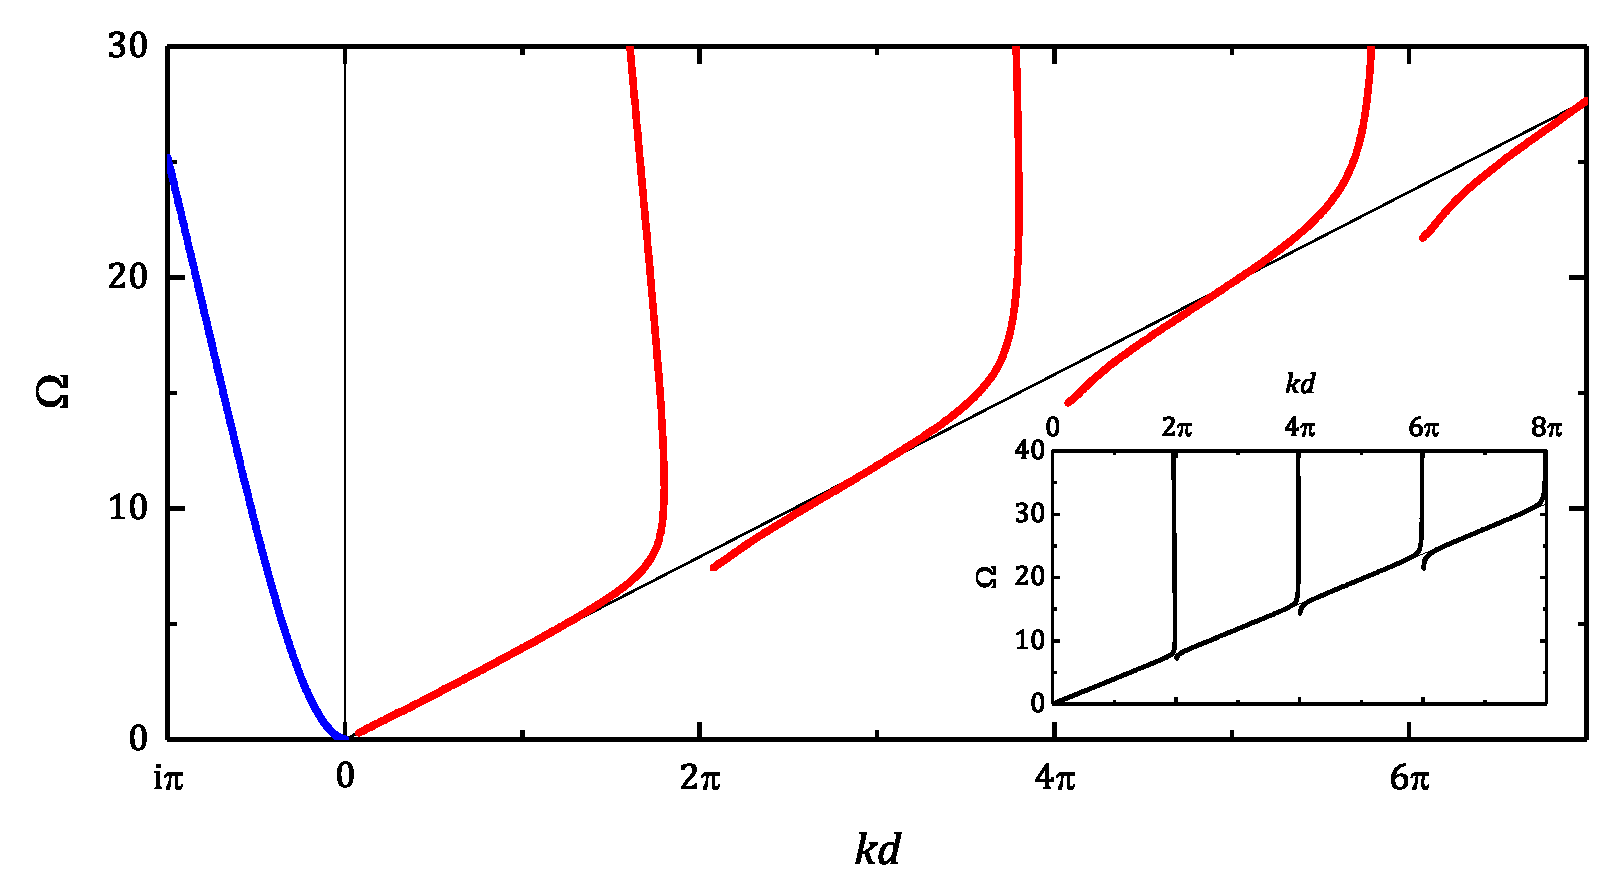
\includegraphics[width=\linewidth]{omega-kd.eps}
\caption{Dispersion relation between dimensionless frequency $\Omega=c_t \omega/d$ and transverse wavevector $kd/2$ obtained from \cref{eq:dispersionXiRayleigh} for the~infinite water channel between two brass plates, $\rho_f/\rho_m = 0.12$. The~linear dispersion for the~case of $\rho_f/\rho_m = 0$ (Rayleigh wave) is shown by a~thin line. The~inset shows the~dispersion of the~fast mode for very weak coupling, $\rho_f/\rho_m = 0.01$. In this case the~waveguide modes are reduced to almost vertical lines at $k d/2 = \pi n$. Dispersion of the~slow mode obtained from \cref{eq:dispersionXiRayleigh} for purely imaginary values of $k$ is plotted to the~left of the~origin.}
\label{fig:spectr}
\end{center}
\end{figure}


The~numerically calculated dispersion of the~real eigenmodes given by \cref{eq:dispersionkRayleigh} is shown in \cref{fig:xi-q} and \cref{fig:spectr}.
The~\cref{fig:xi-q} shows the~dimensionless phase speed $\xi$ versus the~wavevector $q$.
The~fast eigenmodes are enumerated by the~integer $n$, with the~lower number corresponding to the~branch with lower cutoff frequency.
The~slow mode is labeled by $0$.

All the~fast-mode branches lie between the~two horizontal lines, $\xi=c_f/c_t$ and $\xi=1$, and emerge at their corresponding cutoff frequency $\Omega_n$ given by \cref{eq:cutoffRayleigh}.
Close to the~level of the~phase velocity of the~Rayleigh wave, $\xi=\xi_R$, the~dispersion curves flatten and then become steep again.
Eventually, they saturate at the~level $\xi=c_f/c_t$.

The~line displaced below $\xi=c_f/c_t$ in \cref{fig:xi-q} represents the~slow Rayleigh mode.
This branch starts from zero frequency with zero phase speed.
For $q > 5$, the~phase speed already saturates to the~level $\xi=\xi_a$ given by \cref{eq:xiaRayleigh}.
This leaves only the~short subwavelength region, where the~phase speed grows rapidly.
In this region, the~channel width is smaller than the~wavelength of sound, $\lambda \geq 2 \pi d/5$, where the~wavelength is $\lambda=2\pi/\beta=2 \pi d/ q$.

In the~limit of very long wavelengths, $\lambda > 100 \pi d$, the~asymptotic approximation \cref{eq:asymptSlowRayleigh} is valid and agrees well with the~numerically calculated spectrum.

% The~ phase velocity of this mode grows extremely fast, starting from zero and approaching $c_f$ for $q > 5$. The~growth occurs in the~subwavelength region, where the~wavelength $\lambda=2\pi/\beta=2 \pi d/ q$ is  greater than the~channel width, $\lambda \geq 2 \pi d/5$. This narrow subwavelength region is zoomed in the~insert to \cref{fig:xi-q}. Within this region the~frequency $\Omega$ and wavevector $q$ are small parameters. Expansion of \cref{disp} leads to the~following nonlinear dispersion in the~low-frequency limit:
 
%As shown in  \cref{fig:xi-q}, this asymptotics is valid in the~region of very long wavelengths, when $\lambda > 100 \pi d$. It is this part of the~spectrum which provides penetration of sound through {\it any} narrow slit. Unlike transmission through a~channel with ideally rigid walls where the~dispersion is linear (see \cref{symm} for $n =0$), in a~real channel the~vibrations of the~walls result in nonlinear dispersion \cref{dispapprox} with vanishing phase and group velocities in the~low-frequency limit. Analysis of transmission through a~subwavelength acoustic channel will be published elsewhere.

The~\cref{fig:spectr} shows the~dimensionless frequency $\Omega$ versus $kd/2$.
Here the~horizontal axis does not represent the~wavevector in the~direction of propagation, and thus the~slope of the~curves is unrelated to either phase or group velocity.

For $\rho_f/\rho_m \ll 1$, the~dispersion of the~fast modes strictly follows the~linear Rayleigh wave dispersion (given by \cref{eq:dispNoRHSRayleigh}), except for the~points $kd/2=\pi n$ ($n=1,2,\dots$), where the~coupled Rayleigh waves become waveguide modes of the~channel with rigid walls.
The~dispersion curves are practically vertical for those values of $k$.

In the~case of $\rho_f/\rho_m = 0.12$, the~fast-mode branches emerge below the~Rayleigh wave dispersion \cref{eq:dispNoRHSRayleigh} and do not follow the~dispersion curves for either limiting case as accurately as it was for $\rho_f/\rho_m \ll 1$.

%The~asymptotes for the~dispersion branches of the~fast modes are the~linear dispersion of the~Rayleigh wave  and the~waveguide modes
%For almost all values of $kd/2$ the~right-hand side of \cref{eq:dispersionkRayleigh} can be neglected since $\rho_f/\rho_m <<1$. In this approximation \cref{eq:dispersionkRayleigh} gives linear dispersion (Rayleigh wave) which serves as asymptote for the~dispersion curves of the~fast mode. However, near the~points where $kd/2=\pi n$ ($n=1,2,\dots$) the~Rayleigh wave becomes a~waveguide mode of a~channel with rigid walls. Here the~dispersion curves become practically vertical lines as a~result of quantization condition $v_z=\frac{\partial B}{\partial z}|_{z = \pm d/2}=0$. For very small ratio $\rho_f/\rho_m= 0.01$ the~spectrum exhibits this quantization condition with high accuracy, as one can see in the~inset to \cref{fig:spectr}.

The~slow mode is plotted separately since it is characterized by purely imaginary values of $k$ in \cref{eq:dispersionkRayleigh}.
For the~sake of visualization, the~corresponding values of $k$ are plotted along the~negative direction of the~horizontal axis.
When the~value of $k$ is large, $|k|d/2 \gg 1$, the~dispersion of the~slow mode becomes practically linear.


\subsection{Complex Eigenmodes}

The~dispersion equation \cref{eq:dispersionXiRayleigh} has an~infinite number of complex roots with $\re\xi~>~0$ for any frequency $\omega=\Omega d/c_t$ (which is assumed to be purely real).
The~wavevectors $\beta$ of the~corresponding coupled Rayleigh waves acquire imaginary part, $\beta = \omega/c_t\xi = \beta'+i\beta''$.
As a~result, the~eigenmodes either exponentially grow or decay as they propagate into the~channel, as described by the~term $e^{i\beta x}=e^{i\beta'x-\beta''x}$ in the~acoustic potentials.
Since the~exponential growth of the~amplitude is physically unreasonable, only the~roots with $\xi''=\im \xi < 0$ must be considered in order to guarantee that $\beta'' > 0$.

The~decay of the~eigenmode into the~channel implies that the~acoustic energy is radiated away from the~channel (as the~media themselves are lossless).
The~Rayleigh wave in the~solid plates must then be a~propagating wave in $z$-direction, which can be realized if the~coefficients $\nu$ and $\eta$ acquire imaginary parts as well.
Indeed, from the~definitions \cref{eq:nuRayleigh}-\cref{eq:etaRayleigh} it is clear that both $\nu$ and $\eta$ are complex if the~wavevector $\beta$ is complex.
By analyzing the~terms in the~potentials \cref{eq:potLcoupledRayleigh}-\cref{eq:potScoupledRayleigh} that describe the~$z$ dependence, $e^{-\nu z}=e^{-\nu'z-i\nu''z}$ and $e^{-\eta z}=e^{-\eta'z-i\eta''z}$, one can see that the~imaginary parts of both coefficients $\nu$ and $\eta$ must be negative.
Moreover, their real parts need to be negative as well.
The~Rayleigh wave amplitude will then oscillate and exponentially grow along $z$ and oscillate and exponentially decay along $x$.
Such inhomogeneous plane wave is a~so-called leaky wave, which radiates energy in the~direction at a~certain angle from the~channel.
It also maintains constant amplitude along that direction due to the~mutual balancing of the~exponential grow and decay along $z$ and $x$.

It is crucial, however, to specify how the~square roots in these definitions need to be calculated in order to ensure the~desired propagating behavior along $z$.
One way to redefine coefficients \cref{eq:nuRayleigh} and \cref{eq:etaRayleigh} to ensure the~leaky-wave behavior is to choose a~second branch of the~complex square root function:
\begin{align}
\nu~&=~-\sqrt{\beta^2-k_l^2}, &\re\beta \ge k_l=\frac{\omega}{c_l}, \label{eq:numinusRayleigh}\\
\eta~&=~-\sqrt{\beta^2-k_t^2}, &\re\beta \ge k_t=\frac{\omega}{c_t}. \label{eq:etaminusRayleigh}
\end{align}
A~more detailed discussion on the~leaky waves and the~corresponding revision of the~square root function can be found in Appendix \ref{appBranchCut}.

The~dispersion equation for the~coupled Rayleigh leaky modes will then differ from \cref{eq:dispersionXiRayleigh} by having an~additional negative sign in its right-hand side:
\begin{equation}
\label{eq:dispersionXiLeakyRayleigh}
\left(2-\xi^2\right)^2-4\sqrt{1-\xi^2}\sqrt{1-\frac{c_t^2}{c_l^2}\xi^2}
~=~-\frac{\rho_f}{\rho_m}\,\xi^4 \sqrt{\frac{1-\left(c_t/c_l\right)^2\xi^2}{\left(c_t/c_f\right)^2\xi^2-1}}\cot\!\left(\frac{\Omega}{2\xi}\sqrt{\frac{c_t^2}{c_f^2} \xi^2-1}\,\right).
\end{equation}


\begin{figure}
\begin{center}
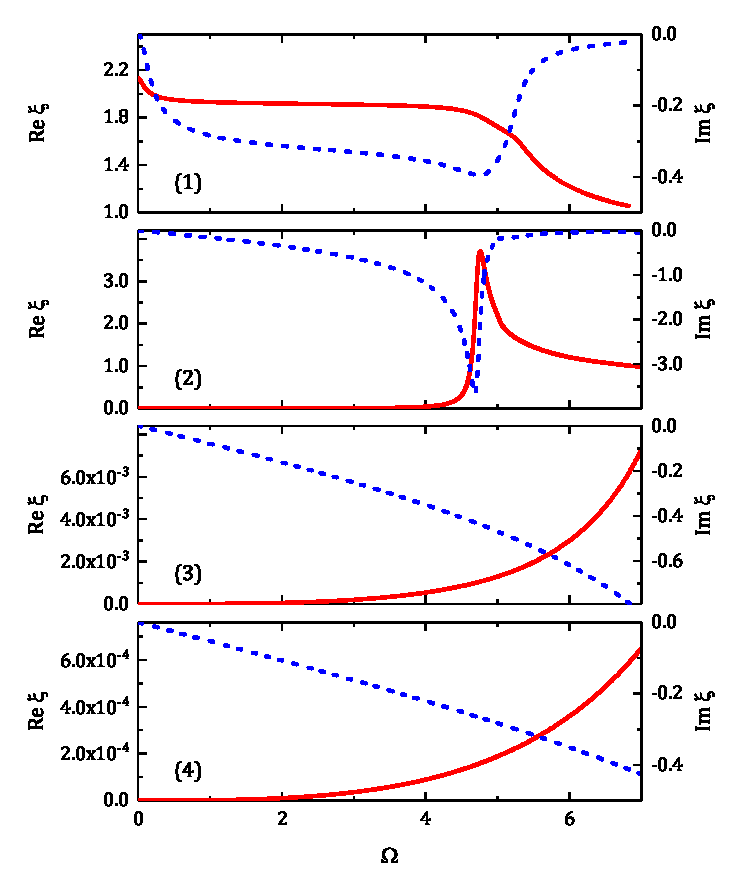
\includegraphics[width=0.85\linewidth]{ComplexRoots.eps}
\caption{Frequency dependence of the~first four complex roots of the~dispersion equation \cref{eq:dispersionXiLeakyRayleigh} for a~water channel between two brass plates. The~real and imaginary parts of each root are shown with solid red and dashed blue curves, respectively.}
\label{fig:roots}
\end{center}
\end{figure}


The~frequency dispersion of several complex roots of \cref{eq:dispersionXiLeakyRayleigh} is shown in \cref{fig:roots}.
These roots are ordered according to their imaginary parts, meaning that they are assigned the~ordinal number $n$ to satisfy the~ordering $
\im\beta_{n} < \im\beta_{n+1}$.
The~first complex root has a~negligible imaginary part at low frequencies.
Because of that, the~corresponding weakly leaky mode contributes to subwavelength transmission of sound through the~metal plates and can compete with the~transmission through the~channel via the~slow Rayleigh mode.

Note that in the~limit of zero channel width there must be a~quasi-longitudinal Rayleigh mode.
Such mode should be only a~slight modification of a~pure longitudinal wave that propagates in the~bulk of the~solid.
Obviously, none of the~real Rayleigh eigenmodes fits this role as their phase speeds are smaller that $c_t$ ($\xi \le 1$).
This means that a~pure longitudinal wave cannot propagate in a~solid plate with a~slit: the~longitudinal vibrations lead to the~inevitable shear displacements in the~solid in the~vicinity of the~slit.
The~corresponding Rayleigh eigenmode must then be necessarily complex and, actually, the~first leaky mode is the~eigenmode in question.
Indeed, in the~limit of zero frequency the~real part of its phase speed approaches $\re\xi = c_l/c_t$, which exactly corresponds to the~speed of longitudinal waves, and its imaginary part vanishes.
Consequently, when considering the~transmission of sound through a~finite sample, the~first leaky mode will be responsible for the~maxima in the~transmission spectrum that would resemble the~Fabry-Perot maxima for the~bulk plate of the~same thickness.

\subsection{Eigenmode Orthogonality}

An~eigenmode (eigenfunction) $f_n$ of a~physical system is always a~nontrivial solution of a~certain \textit{homogeneous} problem, in which there is no external influence on the~system.
The~set of eigenmodes forms a~complete basis in the~function space.
Then any process (given by a~function $f$) occurring in the~system can be represented as a~superposition of the~eigenmodes, or in other words, it can be expanded over the~known basis:
\begin{equation}
\label{eq:basisRayleigh}
f~=~\sum C_n f_n.
\end{equation}
The~coefficients of the~expansion can easily be found if the~eigenmodes are orthogonal:
\begin{equation}
\langle f_n, f_m \rangle~=~||f_n||^2\delta_{n,m}.
\end{equation}
Here the~term in the~left-hand side is a~generalized inner product of two eigenmodes, $||\cdot||$ gives the~norm of its argument, and $\delta_{n,m}$ is the~Kronecker symbol.
The~coefficients of the~expansion $C_m$ are then immediately obtained as
\begin{equation}
C_m~=~\frac{\langle f, f_m\rangle}{||f_m||^2}.
\end{equation}

For the~problem of sound transmission through a~finite-sized fluid channel between two metal plates, determining the~unknown coefficients in the~expansion of the~signal over the~coupled Rayleigh modes will be crucial for obtaining the~solution.
However, the~Rayleigh eigenmodes are not orthogonal, for the~reason that the~boundary conditions at the~fluid-solid interface \cref{eq:coeffRelationsRayleigh} explicitly contain the~wavevector $\beta$ \cite{bobrovnitskii}.
Moreover, the~eigenmodes of any problem where the~elastic waves are confined to a~finite volume are known to be nonorthogonal.
For example, the~Lamb waves (normal vibrations) in an~elastic slab are not mutually orthogonal over the~slab width \cite{lyon}.
Even though a~lot of efforts were put to redefine the~orthogonality for Lamb waves from the~reciprocity principles \cite{bobrovnitskii,achenbac,zakharov,folk}, the~proposed new relations do not facilitate calculating the~coefficients of the~expansion $C_m$. 

The~nonorthogonal basis can always be transformed into an~orthogonal one by, e.g., employing the~Gram-Schmidt procedure, however, I will not be using this procedure for several reasons.
One of them is that this orthogonalization process is quite difficult to perform in regards to the~Rayleigh eigenmodes, and using it would significantly increase the~complexity of the~problem.
Another reason is that it will be much easier to calculate the~unknown coefficients $C_m$ if one expands both the~function $f$ and the~eigenmodes $f_n$ over some simple orthogonal basis $g_n$:
\begin{equation}
f~=~\sum f^{(m)}g_m, \qquad f_n~=~\sum f_n^{(m)}g_m,
\end{equation}
with the~coefficients $f^{(m)}$ and $f_n^{(m)}$, respectively. 
After substituting the~latter relations to \cref{eq:basisRayleigh} and calculating the~inner product with every $g_m$ for each part of the~equation, the~following set of equations is obtained:
\begin{equation}
f^{(m)}~=~\sum C_n f_n^{(m)}.
\end{equation}
The~linear system can now be solved numerically, for example.
This discussion clearly shows that the~use of the~nonorthogonal basis is not too much of an~inconvenience in solving a~problem.

%It is well-known that an~eigenvalue problem for elastic waves in a~finite volume leads to a~set of nonorthogonal eigenfunctions. In particular, normal vibrations of elastic plate (Lamb waves) are not orthogonal over the~width of the~plate \cite{lyon}.  While several "orthogonality relations" for Lamb waves based on the~reciprocity relations have been proposed \cite{bobrovnitskii,achenbach}, they (or their modification for solid-fluid structure \cite{zakharov}) cannot help in calculation of $b_n^{\pm}$.

%The~right-hand-sides of Eqs. \cref{eq:app_22} and \cref{eq:app_23} are presented in the~form of expansions over eigenfunctions of vibrating fluid channel. These eigenfunctions are defined on the~semiaxis $z>0$. They are oscillating, $\cos(k_nz)$, within the~channel, $0<z<d/2$, and evanescent, $\exp(-\eta_n z)$, $\exp(-\nu_n z)$, inside the~metal plates, $z> d/2$. These eigenfunctions, as well as the~displacements and velocities defined by them, are not orthogonal. The~lack of orthogonality is due to the~boundary conditions at $z= \pm d/2$, explicitly containing the~eigenvector $\beta_n$, as it was mentioned in Ref. \cite{bobrovnitskii} with respect to non-orthogonality of Lamb modes in a~solid plate.

%While the~non-orthogonal basis does not allow analytical calculation of the~unknowns $b_n^{\pm}$, it really does not impose additional difficulty in numerical calculation. \textbf{On the~contrary, using orthogonal basis would be less appropriate, because orthogonalization of the~naturally introduced non-orthogonal basis of channel eigenfunctions is itself a~procedure of greater difficulty than solving an~inhomogeneous system of linear equations in the~method shown below}. Due to the~fact that the~size of the~set of equations \cref{eq:app_22} and \cref{eq:app_23} is cut by the~number of calculated roots $\xi_n(\omega)$, $n =1,2,\dots, N$, the~necessary set of equations for $b_n^{\pm}$ can, for example, be obtained by equating the~first $N$ Fourier coefficients of the~both sides of Eqs. \cref{eq:app_22} and \cref{eq:app_23}. We introduce the~finite Fourier transform defined on a~segment $0<z<R_d$.

% to stress that the~Fabry-Perot maxima in transmission are due to the~roots which are necessary complex. Indeed, these maxima appear when longitudinal waves interfere constructively at the~length $h$. Since $c_l>c_t$, the~roots of the~dispersion equation which correspond to the~phase velocities close to $c_l$ cannot lie within the~interval $0<\xi \leq 1$ (where all the~real roots lie), i.e. they are all complex. This complexity reflects an~obvious fact that in a~solid plate with a~slit pure longitudinal waves cannot propagate. Even a~narrow slit gives rise to shear displacements which change the~amplitude and phase of the~Fabry-Perot resonance. The~imaginary part of the~quasi-longitudinal solution may be quite small which means only slight modification of the~Fabry-Perot resonance. For example, the~complex root shown in Fig.~\cref{fig:roots} has the~real part close to 2 (which is approximately the~ratio $c_l/c_t$ in brass) and negligible imaginary part in the~limits of either zero frequency or zero channel width. This root corresponds to quasi-longitudinal sound wave propagating in metal.


%%%%%%%%%%%%%%%%%%%%%%%%%%%%%%%%%%%%%%%%%%%%%%%%
%%%%%%%%%%%%%%%%%%%%%%%%%%%%%%%%%%%%%%%%%%%%%%%%
%%%%%%%%%%%%%%%%%%%%%%%%%%%%%%%%%%%%%%%%%%%%%%%%
%%%%%%%%%%%%%%%%%%%%%%%%%%%%%%%%%%%%%%%%%%%%%%%%
% A~solution of the~wave equation in the~fluid and in the~plates can be written as a~superposition of the~corresponding eigenmodes \cref{pot}. Linear relations between the~coefficients $b_n$, $l_n$, and $s_n$ are obtained from the~boundary conditions. Since the~channel is infinite we can consider only the~waves propagating in positive direction of axis $x$ and omit super-indices $\pm$.
%
%At the~fluid-metal interface $z=d/2$ 
%Here $\sigma_{ik}(x,z)$ is the~stress tensor in the~elastic plates.
%%and it was taken into account that the~stress tensor for ideal fluid is diagonal,
%%$\sigma^{(f)}_{ik}=-p\delta_{ik}$.
%Using the~Hooke's Law $\sigma_{ik}~=~\lambda u_{ll}\delta_{ik} + 2\mu u_{ik}$
%the~nonzero components of the~stress tensor can be expressed through the~potentials
%\begin{align}
%\label{8}
%\sigma_{xx}~&=~-\lambda k_l^2 L +2\mu\left(\frac{\partial^2 L}{\partial x^2}-\frac{\partial^2 S}{\partial x \partial z}\right), \\
%\sigma_{zz}~&=~-\lambda k_l^2 L +2\mu\left(\frac{\partial^2 L}{\partial z^2}+\frac{\partial^2 S}{\partial x \partial z}\right), \notag \\
%\sigma_{xz}~&=~\mu\left(2\frac{\partial^2 L}{\partial x \partial z}+\frac{\partial^2 S}{\partial x^2}-\frac{\partial^2 S}{\partial z^2}\right). \notag
%\end{align}
%Here $\lambda$ and $\mu$ are the~Lam{\'e} coefficients, $\mu~=~\rho_m c_t^2, \,\, \lambda+2\mu~=~\rho_m c_l^2$. Substituting the~potentials  \cref{pot} to \cref{8} and \cref{dispvec}, the~components of $\sigma_{ik}$ and $\bf u$ are expressed through the~unknown constants $l_n$ and $s_n$.  The~velocity ${\bf v} = \nabla B$ and the~pressure $p=i\omega \rho B$ are expressed through $b_n$. Thus, all the~dynamical variables are given in terms of three unknowns, $l$, $s$, and $b$.

%The~boundary conditions \cref{7} written in terms of $l$, $s$, and $b$ (here sub-index $n$ can be omitted) lead to the~following set of linear equations:
%\begin{equation}
%\label{10}
%\left\{
%\begin{aligned}
%&\left(2\mu\nu^2-\lambda k_l^2\right)\,e^{-\nu d/2}\cdot l
%- 2i\mu \eta \beta\,e^{-\eta d/2}\cdot s+i\omega\rho_f \cos(k d/2)\cdot b~&=~0, \\
%&2i\nu \beta \,e^{-\nu d/2}\cdot l+ e^{-\eta d/2}\left(\beta^2 +\eta^2 \right) \cdot s ~&=~0, \\
%&k \sin(k d/2)\cdot b+i\omega\nu \,e^{-\nu d/2}\cdot l +\omega\beta \,e^{-\eta d/2}\cdot s~&=~0.
%\end{aligned}
%\right.
%\end{equation}
%This set has nontrivial solution if the~corresponding determinant vanishes, viz
%\begin{equation}
%\label{11}
%\left(\eta^2+\beta^2\right)^2-4\nu\eta\beta^2~=~\frac{\rho_f}{\rho_m}\frac{\omega^4}{c_t^4}\frac{\nu}{k}\,\cot \frac{kd}{2}.
%\end{equation}
%Here $k$, $\nu$, and $\eta$ are expressed through $\omega$ and $\beta$ using \cref{kk}.
%Dependence on the~channel width $d$ can be eliminated if dimensionless frequency $\Omega = \omega d/c_t$ and wave vector $q = \beta d$ are introduced.
%\begin{equation}
%\label{disp2}
%\left(2 q^2-\Omega^2\right)^2 - 4 q^2 \sqrt{q^2 - (c_t/c_l)^2 \Omega^2} \sqrt{q^2 - \Omega^2} 
%~=~ \frac{\rho_f}{\rho_m}\Omega^4 \sqrt{\frac{q^2 - (c_t/c_l)^2 \Omega^2}{(c_t/c_f)^2 \Omega^2 - q^2}}\,\cot( \frac{1}{2}\sqrt{\frac{c_t^2}{c_f^2} \Omega^2 - q^2}).
%\end{equation}
%Dispersion relation \cref{disp} for the~phase velocity $\xi$ is obtained from \cref{disp2} by substitution $q=\Omega /\xi$. Real and complex solutions of \cref{disp2} define the~allowed values of the~wave vector $q_n= q_n(\Omega)$ for each frequency $\Omega$.




%Expansions \cref{pot} of the~potentials over eigenmodes can be used if all real roots and sufficient number of complex roots of the~dispersion equation \cref{disp} are known. In general case each root depends on frequency, $\xi_n=\xi_n(\omega)$ that shows frequency dispersion of the~corresponding mode. Examples of frequency dispersion for the~lowest two real solutions are given in the~left panel in \cref{fig:roots}. The~mode which starts at $\omega = 0$ is the~slow mode (blue line). It exhibits strong dispersion in the~subwavelength regime and at $\omega > 0.5$ MHz the~phase velocity saturates at the~level $\xi=c_f/c_t$, i.e the~slow mode becomes dispersionless sound wave, propagating with speed $c_f$. Red line shows dispersion of the~first waveguide mode. This mode starts at cut-off frequency $(c_t/d) \Omega_1$. 


%%%%%%%%%%%%%%%%%%%%%%%%%%%%%%%%
%{The~eigenmodes in  \cref{pot} are labeled by integer $n$ which numerates the~roots of the~dispersion equation $\beta_n = \beta_n(\omega)$. This equation is derived in Appendix \ref{appRayleigh} from the~continuity of force and velocity at the~boundaries $z= \pm d/2$ \cite{adv,Lloyd}. Since the~system is symmetric with respect to the~plane $z=0$ the~eigenmodes are either even or odd functions of $z$. Odd modes are excited at oblique incidence or if the~plates are made of different metals \cite{channel1}. In our case only even modes can be excited. The~dispersion equation for these modes is written as follows:
%\begin{equation}
%\label{disp}
%\left(2-\xi^2\right)^2-4\sqrt{1-\xi^2}\sqrt{1-\frac{c_t^2}{c_l^2}\xi^2}
%~=~\pm\frac{\rho_f}{\rho_m}\,\xi^4 \sqrt{\frac{1-\left(c_t/c_l\right)^2\xi^2}{\left(c_t/c_f\right)^2\xi^2-1}}\cot\!\left(\frac{\omega}{\xi}\frac{d}{2c_t}\sqrt{\frac{c_t^2}{c_f^2} \xi^2-1}\,\right).
%\end{equation}
%Here $\rho_m$ is the~density of the~elastic plates plates. Each root $\xi_n$ of the~dispersion equation gives the~normalized phase velocity $\xi_n = \omega/ c_t \beta_n$ of the~coupled quasi-surface waves. Since the~coupling between these  waves occurs through the~fluid, the~r.h.s of \cref{disp} is proportional  to the~ratio $\rho_f/\rho_m$. When $\rho_f/\rho_m = 0$ the~vibrations of the~plates are uncoupled and \cref{disp} is reduced to the~well-known cubic equation with respect to $\xi^2$. Its unique solution $\xi = \xi_R$ defines the~velocity of dispersionless surface Rayleigh wave at the~plane interface between vacuum and elastic solid \cite{viktor}.}
%
%{The~dispersion equation has finite number of real roots
%and infinite number of complex roots with  $\mathrm{Re}\xi_n > 0$. {\bf Due to the~factor $\sqrt{1-\xi^2}$ all real roots lie within the~interval $0<\xi \leq 1$.} The~real roots are obtained from  \cref{disp} with "+" sign in the~right-hand side. Each complex root  gives rise to an~inhomogeneous plane wave in the~expansions \cref{pot}. These terms oscillate and decay with the~coordinate $z$. For complex roots the~decrements $\nu_n$ and $\eta_n$ acquire imaginary parts, which must be negative  in order the~corresponding modes run {\it away} from the~channel. This scattering condition is satisfied for the~roots with $\mathrm{Im}\xi_n < 0$, which are obtained from \cref{disp} with "-" sign in the~right-hand side. For each
%frequency $\omega$ all the~real roots must be included in the~expansions \cref{pot}. The~number of complex roots included in numerical calculations depends on
%desired accuracy. The~roots are arranged in ascending order of the~imaginary part of the~longitudinal wave vector $\beta_n = \omega/(c_t \xi_n)$ ($|\mathrm{Im} \beta_{n-1}| < |\mathrm{Im} \beta_n|$), since those with smaller $|\mathrm{Im} \beta|$ give larger contributions.  For infinitely long channel the~complex solutions should be ignored as they decay exponentially with length, but they play essential role in sound transmission through a~finite-length channel.}

%{Solutions of the~transcendental equation \cref{disp} are obtained numerically. For channel of width $d$ \cref{disp} gives implicit relation between the~dimensionless phase velocity $\xi$ and frequency $\omega$. Substituting $\omega = (c_t/d)\xi q$, where $q=\beta d$ is dimensionless wave vector, into the~argument of cotangent in \cref{disp}, we obtain equation which relates the~dimensionless phase velocity $\xi$ and wave vector $q$. This equation is independent of the~channel width $d$ and it leads to the~spectrum shown in \cref{fig:xi-q}.
% The~spectrum consists of two unequal parts. One is so-called {\it fast mode} propagating faster than sound wave in the~fluid, $\xi>c_f/c_t$. It has infinite number of branches (shown in red) which originate from the~symmetric waveguide modes
%\begin{equation}
%\label{symm}
%\omega_n = c_f \sqrt{\left(\frac{2\pi n}{d}\right)^2+\beta^2}, \,\,\, n = 0,1,2,\dots
%\end{equation}
%of a~channel with ideally rigid walls, $\rho_m, c_t \rightarrow \infty$. More detailed analysis of the~spectrum in the~limit $\rho_f/\rho_m \rightarrow 0$ is given in Appendix \ref{appRayleigh}. All the~branches of the~fast mode lie between two horizontal lines, $c_f/c_t < \xi \leq 1$. Unlike the~waveguide spectrum \cref{symm} where each phase velocity $\omega_n/\beta$ diverges at $\beta = 0$, except the~mode with $n = 0$, in a~channel with elastic boundaries all fast modes start with finite phase velocity $\xi = 1$ at the~wavevector
%\begin{equation}
%\label{veloc}
%Q_n = \beta_n d= \frac{2}{\sqrt{(c_t/c_f)^2 -1}} \left[ \pi n +
%\arctan\left(\frac{\rho_f}{\rho_m} \sqrt{\frac{1-(c_t/c_l)^2}{(c_t/c_f)^2-1}}\, \right)\right] ,\,\, n = 0,1,2, \dots
%\end{equation}
%Near the~point where each branch crosses the~level of the~phase velocity of the~Rayleigh wave, $\xi=\xi_R$, the~slope of the~dispersion curve noticeably decreases since for the~parameters used in the~plot of \cref{fig:xi-q} the~ratio  $\rho_f/\rho_m=0.12$ is quite small.}
%
%{Another part of the~spectrum in \cref{fig:xi-q} is represented by a~blue line. It is displaced below the~level $\xi=c_f/c_t$, i.e. this mode propagates slower than sound in the~fluid. The~right-hand side of the~dispersion equation \cref{disp} remains real while the~square root $\sqrt{(\frac{c_t}{c_f})^2 \xi^2 -1}$ is pure imaginary. The~ phase velocity of this mode grows extremely fast, starting from zero and approaching $c_f$ for $q > 5$. The~growth occurs in the~subwavelength region, where the~wavelength $\lambda=2\pi/\beta=2 \pi d/ q$ is  greater than the~channel width, $\lambda \geq 2 \pi d/5$. This narrow subwavelength region is zoomed in the~insert to \cref{fig:xi-q}. Within this region the~frequency $\Omega$ and wavevector $q$ are small parameters. Expansion of \cref{disp} leads to the~following nonlinear dispersion in the~low-frequency limit:
%\begin{equation}
%\label{dispapprox}
%\Omega \approx {\sqrt{\frac{\rho_m}{\rho_f}\left(1-\frac{c_t^2}{c_l^2}\right)}}\, (\beta d)^{3/2}.
%\end{equation}
%As shown in  \cref{fig:xi-q}, this asymptotics is valid in the~region of very long wavelengths, when $\lambda > 100 \pi d$. It is this part of the~spectrum which provides penetration of sound through {\it any} narrow slit. Unlike transmission through a~channel with ideally rigid walls where the~dispersion is linear (see \cref{symm} for $n =0$), in a~real channel the~vibrations of the~walls result in nonlinear dispersion \cref{dispapprox} with vanishing phase and group velocities in the~low-frequency limit. Analysis of transmission through a~subwavelength acoustic channel will be published elsewhere. It is noteworthy to mention that transmission of electromagnetic waves through a~deeply subwavelength metallic slit also exhibits interesting features which do not exist for perfectly conducting screens \cite{Seo,Xia}}.


%%%%%%%%%%%%%%%%%%%%%%%%%%%%%%%%%%%%%%%%%%%%%%%%%%%%%%%%%%%%%%%%%%%%
\section{Scattering Problem}

The~knowledge of the~eigenmodes of the~infinite fluid channel allows to tackle the~problem of sound transmission through a~finite sample.
Namely, the~acoustic field inside the~channel and the~plates can be now expressed as a~superposition of the~channel eigenmodes.
In this approach the~boundary conditions at the~channel walls are automatically satisfied.
Also, one obtains a~practically exact analytical solution since the~acoustic potentials account for the~\textit{total} field at any given point.

The~only limiting factor here is the~number of the~eigenmodes used in the~potentials expansion.
The~exact solution requires writing an~infinite series over all possible eigenmodes.
Practically, the~series in question converges quite fast and it is sufficient to consider only the~first few of the~coupled Rayleigh eigenmodes.

\subsection{Geometry}

I will be considering a~problem that closely imitates the~conditions of the~experiment reported in \cite{channel1}.
In this experiment, two brass or aluminum plates of length $L=12$ cm and thickness $h$ were separated by a~distance $d$ (the~slit aperture).
The~system was immersed in a~water tank, and two transducers
of diameter $2R_d=1.5^{\prime\prime}$ were used to produce and detect the~sound.
Both transducers were positioned at a~distance $l=8$ cm from the~plates, centered with respect to the~channel, and the~sound was incident normally on the~slit.
This experimental setup is schematically shown in \cref{fig:geometryRayleigh}, as well as the~values of $d$ and $h$ for which the~experiment was performed.
Note that the~gravity is acting along the~$y$-direction.
Any effect of gravity is, however, omitted and the~problem is assumed uniform along the~$y$-axis.

\begin{figure}
\begin{center}
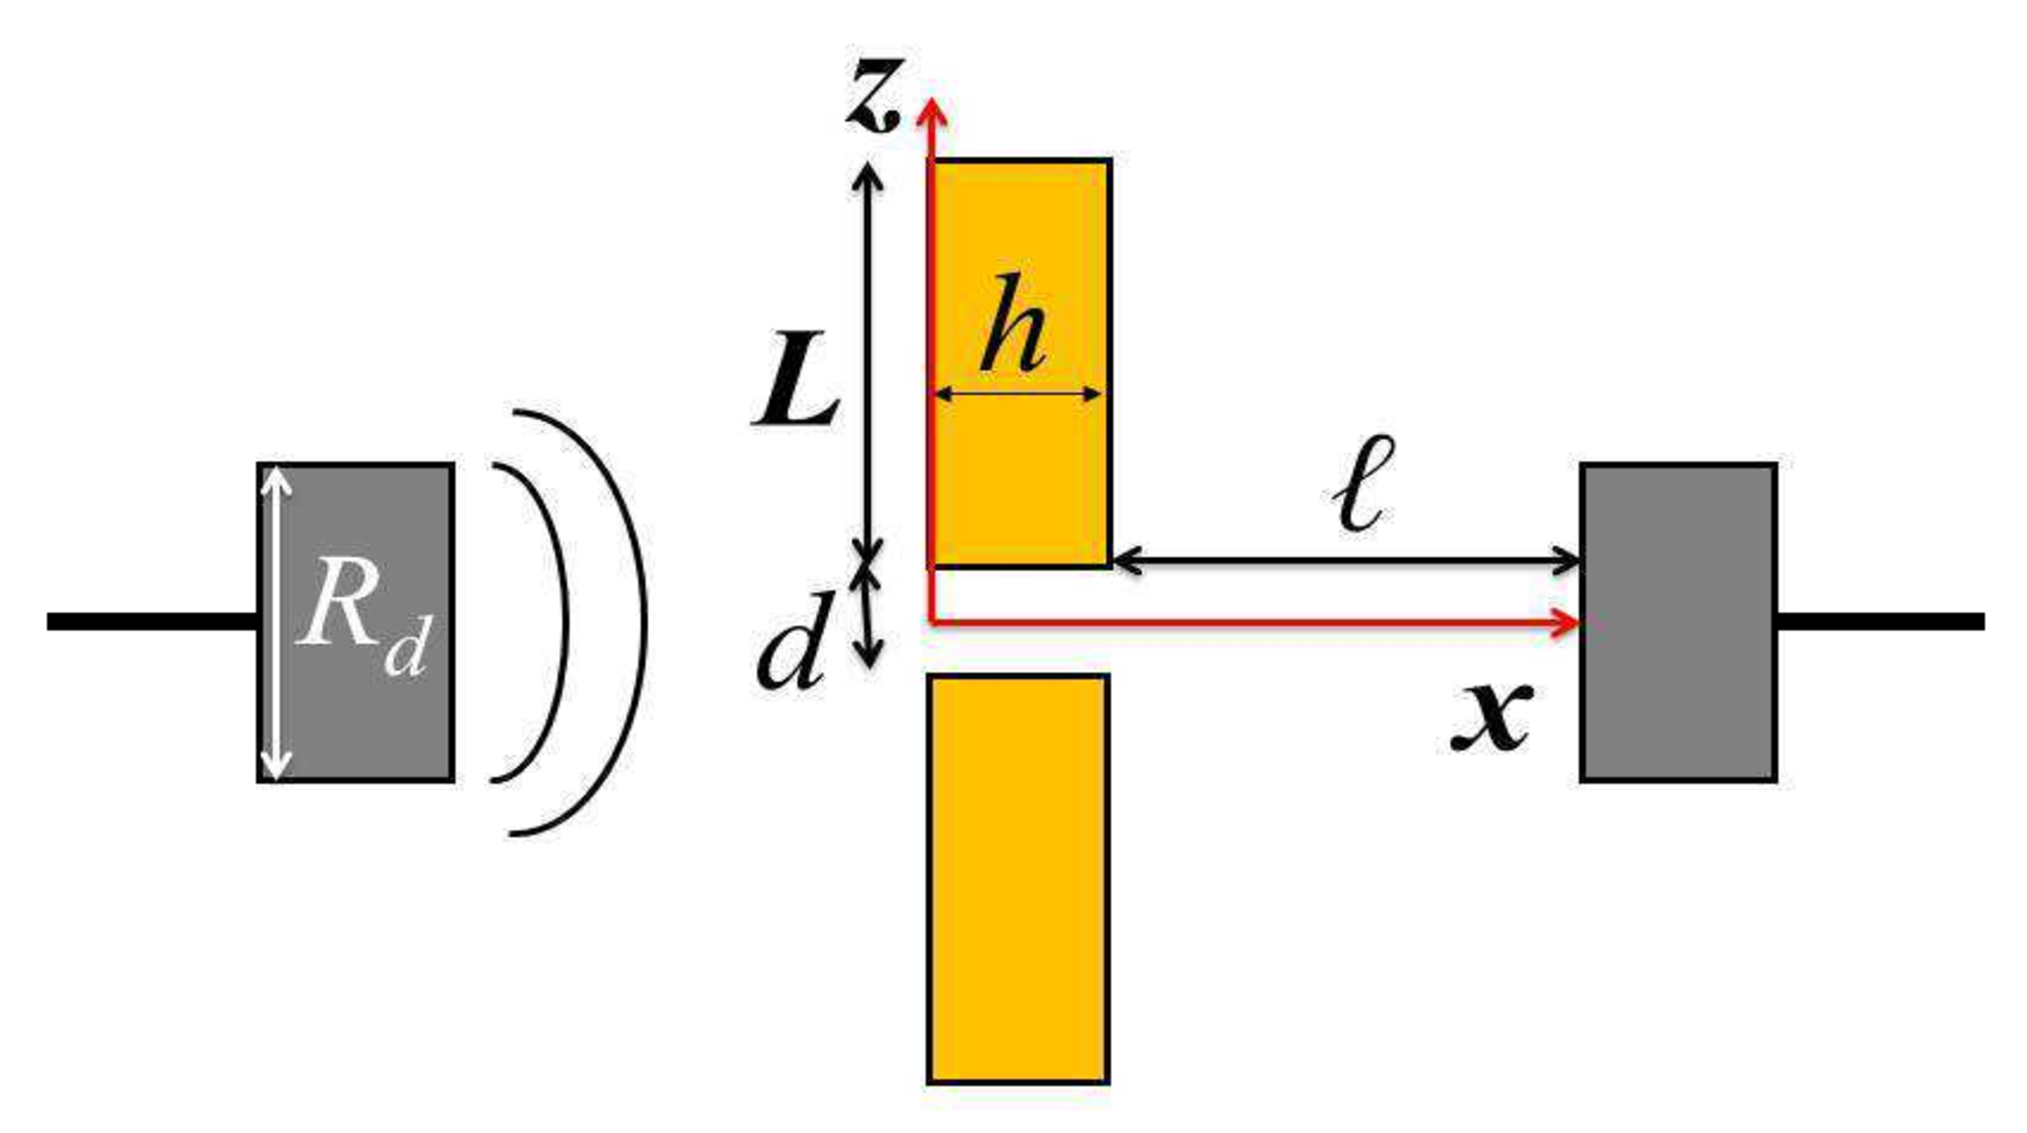
\includegraphics[width=0.85\linewidth]{fig0_geometry.eps}
\caption{Experimental setup showing the~geometrical parameters of the~fluid channel between the~metal plates and the~configuration of transducers.}
\label{fig:geometryRayleigh}
\end{center}
\end{figure}

Since the~size of each transducer is much larger than the~channel width, $d \ll R_d$, I will model the~incoming sound by a~plane wave. 


% a~sound wave was generated and detected by two $1.5^{\prime\prime}$ transducers immersed in a~water tank at equal distance  $l=8$ cm from the~plates. A~slit between two square brass or aluminum plates with side $L = 12$ cm is located in front of the~ transducers. A~sound wave was incident normally to the~slit and the~transmission spectrum was measured with compensation of the~non-flat frequency response of the~piezoelectric transducers. The~plate thickness $h$ defines the~length of the~water channel and its width $d$ (the~slit's aperture) is maintained by means
%of a~sample holder that fixes both metal plates. This experimental setup is schematically shown in the~inset to \cref{fig:experimentRayleigh}.

\subsection{Acoustic Potentials of Transmitted and Reflected Waves}

The~plane acoustic wave that is normally incident on the~slit and the~plates from the~left is described by the~acoustic potential $(p_0/i \omega \rho_f) \exp(ik_fx-i\omega t)$.
The~reflected and the~transmitted acoustic fields are denoted as $R(x,z)$ ($x<0$) and $T(x,z)$ ($x>h$), respectively.
Since the~channel scatters the~sound in every possible direction, I write the~potentials $R(x,z)$ and $T(x,z)$ as Fourier integrals
\begin{align}
R(x,z)~&=~\int\limits_{-\infty}^{+\infty}r(k)e^{ikz-i\beta(\!k)x}dk, &x \leq 0, \label{refl}\\
T(x,z)~&=~\int\limits_{-\infty}^{+\infty}t(k)e^{ikz+i\beta(\!k)(x-h)}dk , &x \geq h, \label{transm}
\end{align}
where the~amplitudes $r(k)$ and $t(k)$ are
\begin{align}
r(k)~&=~\frac{1}{2\pi}\int\limits_{-\infty}^{+\infty}R(0,z)e^{-ikz}dz, \label{refl2}\\
t(k)~&=~\frac{1}{2\pi}\int\limits_{-\infty}^{+\infty}T(h,z)e^{-ikz}dz. \label{transm2}
\end{align}
The~longitudinal (along $x$) component of the~wave vector is defined as $\beta(k)=\sqrt{k_f^2-k^2}$ for $|k| < k_f$ and $\beta(k)=i\sqrt{k^2-k_f^2}$ for $|k| > k_f$.
Each Fourier integrals essentially represents a~combination of all possible plane ($|k| < k_f$) and evanescent ($|k| > k_f$) waves that contribute to either reflection or transmission.


%To calculate the~transmission of a~plane sound wave coming from the~left, $(p_0/i \omega \rho_f) \exp(ik_0x-i\omega t)$, we introduce the~potentials of the~reflected $R(x,z)$ ($x<0$) and transmitted $T(x,z)$ ($x>h$) acoustic fields. They define velocity and pressure in the~fluid (e.g. ${\bf v} = \nabla R$, $p = p_0+ i \omega \rho_f R$ for $x<0$). Here  $k_0=\omega / c_f$,  $\rho_f$ is the~density and $c_f$ is the~speed of sound in the~fluid.  The~potentials of the~reflected and transmitted fields are represented through their Fourier integrals
%\begin{equation}
%R(x,z)~=~\int\limits_{-\infty}^{+\infty}r(k)e^{ikz-i\beta(\!k)x}dk , \,\,\, x \leq 0,
%\label{refl}
%\end{equation}
%\begin{equation}
%\label{trans}
%T(x,z)~=~\int\limits_{-\infty}^{+\infty}t(k)e^{ikz+i\beta(\!k)(x-h)}dk , \,\,\, x \geq h.
%\end{equation}
%Here the~longitudinal (along $x$) component of the~wave vector is defined as $\beta(k)=\sqrt{k_0^2-k^2}$ for $|k| < k_0$ and $\beta(k)=i\sqrt{k^2-k_0^2}$ for $|k| > k_0$.
%The~Fourier components $r(k)$ and $t(k)$ are linearly related through the~boundary conditions.

In the~region $0 \leq x \leq h$, i.e., inside the~fluid channel and the~elastic plates, the~potentials are superpositions of forward and backward propagating eigenmodes of the~corresponding infinite channel:
\begin{align}
B(x,z)~&=~\sum\limits_{n} (b_n^+ e^{i\beta_nx}+b_n^- e^{-i\beta_nx})\cos{k_nz}, &|z| < d/2, \label{pot1} \\
L(x,z)~&=~\sum\limits_{n}({l_n^+}e^{i\beta_nx}+l_n^- e^{-i\beta_nx})e^{-\nu_n|z|}, &|z| > d/2, \label{pot2} \\
S(x,z)~&=~\sum\limits_{n}({s_n^+}e^{i\beta_nx}-{s_n^-}e^{-i\beta_nx})e^{-\eta_n|z|}, &|z| > d/2. \label{pot3}
\end{align}
The~summation runs over all possible eigenmodes (propagating and leaky) of the~system for a~given frequency.
The~superindices "$+$" and "$-$" indicate propagation in the~$+x$ or $-x$ direction.
The~potentials for the~backpropagating Rayleigh waves are obtained from those describing the~propagation forward by applying the~symmetry transformation $x\rightarrow -x$, $y\rightarrow -y$, which is essentially the~$180^{o}$ rotation around the~$z$-axis.

The~unknown amplitudes $t(k)$ and $r(k)$ in \cref{refl}-\cref{transm} and the~coefficients $b_n$, $l_n$, and $s_n$ in \cref{pot1}-\cref{pot3} can be determined after the~appropriate boundary conditions at both vertical ($x=0,h$) surfaces of the~structure are established.
%where ${B}$ is the~ velocity potential of the~fluid (${\bf v}(x,z)=\nabla B$, $|z| \leq d/2$) and the~potentials $L$ and $S$ give the~displacement vector in the~plates,
%\begin{equation}
%\label{dispvec}
%{\bf u}=\nabla L + \nabla \times (S {\bf \hat y}), \,\,\, |z| \geq d/2.
%\end{equation}
%The~transversal parts of the~wave vectors in the~fluid and in the~plates are defined as
%\begin{align}
%\label{kk}
%&k_n=\sqrt{k_0^2-\beta_n^2}, \\
%&\nu_n=\sqrt{\beta_n^2-k_l^2}, \notag \\
%&\eta_n=\sqrt{\beta_n^2-k_t^2},\notag
%\end{align}
%where $\mathrm{Re}\,(\nu_n,\eta_n)>0$, $k_{l,t}=\omega/c_{l,t}$, and $c_t$  ($c_l$) is the~speed of transversal (longitudinal) sound in the~plates.
%%Summation in \cref{pot} runs over the~roots of the~dispersion equation, both real and complex. 
%Our final goal is calculation of the~reflected and transmitted acoustic fields in the~fluid.
%%%%%%%%%%%%%%%%%%%%%%%%%%%%%%%%%%%%%%%%%%%%%%%%%%%%%%%%%%%%%%%%%%%%%%%%%%%%%%%%%%%%%%%%%%%%%%%%%%%%%%%%%%%%%%%%%%%%%%%%%%%%%%%%%%%%%%%%%%%%%%%%%%%%%%%%%%%
%                                                      FIGURE #2
%%%%%%%%%%%%%%%%%%%%%%%%%%%%%%%%%%%%%%%%%%%%%%%%%%%%%%%%%%%%%%%%%%%%%%%%%%%%%%%%%%%%%%%%%%%%%%%%%%%%%%%%%%%%%%%%%%%%%%%%%%%%%%%%%%%%%%%%%%%%%%%%%%%%%%%%%%%
%\begin{figure}
%\begin{center}
%%\includegraphics[width = 9cm]{fig2.eps}
%\caption{ Dimensionless phase velocity $\xi=\Omega/q$ vs wave vector $q=\beta d$ for infinite brass channel filled by water. Fast mode is presented by infinite number of waveguide branches above the~speed of sound in water, $c_f/c_t< \xi < 1$ (red curves). Phase velocity of the~slow mode grows very fast (blue line near the~vertical axis) and saturates at the~level $\xi= c_f/c_t$ for very small $q= \beta d \approx 0.2$. Insert is the~blowup of this narrow region where the~phase velocity behaves as $\xi \sim \sqrt{qd}$. Dashed line is asymptotic dependence obtained from \cref{dispapprox}. }
%\label{fig:xi-q}
%\end{center}
%\end{figure}
%--------------------------------------------------------------------------------------------------------------------------------------------------------------



%%%%%%%%%%%%%%%%%%%%%%%%%%%%%%%%%%%%%%%%%%%%%%%%%%%%%%%%%%%%%%%%%%%%
\subsection{Solution of the~Scattering Problem}

The~coefficients $l_n^{\pm}$, $s_n^{\pm}$, and $b_n^{\pm}$ describe a~particular coupled Rayleigh wave, so the~relationship between them is established by \cref{eq:coeffRelationsRayleigh}, namely,
\begin{align}
{l_n^{\pm}}&=-\frac{i k_n c_t^2}{\nu_n\omega^3}(\eta_n^2+\beta_n^2)\sin\frac{k_nd}{2}e^{\nu_n\!d/2}\,{b_n^{\pm},} \label{eq:lbRayleigh} \\
{s_n^{\pm}}&=-\frac{2 k_n\beta_n c_t^2}{\omega^3}\sin\frac{k_nd}{2}e^{\eta_n\!d/2}\,{b_n^{\pm}}. \label{eq:sbRayleigh}
\end{align}

Both \cref{eq:lbRayleigh} and \cref{eq:sbRayleigh} can now be used to eliminate the~unknown coefficients $l_n^{\pm}$ and $s_n^{\pm}$ of the~acoustic potentials in plates from all subsequent calculations.
The~remaining unknowns $t(k)$, $r(k)$, and $b_n^{\pm}$ need to be related via the~boundary conditions at the~vertical boundaries $x=0$ and $x=h$ that were not used so far.
These four conditions for velocity and pressure are as follows:
\begin{align}
p_0+i \omega \rho_f \left.R(x,z)\right|_{x=0} &= \left[
\begin{aligned}
i \omega \rho_f B&\left.(x, z)\right|_{x=0}, &|z| < d/2, \\
\sigma_{xx}&\left.(x,z)\right|_{x=0}, &|z| > d/2,
\end{aligned}
\right. \label{eq:bc12Rayleigh} \\
%%%%%%%
\frac{p_0}{\rho_f c_f}+\left.\frac{\partial R(x,z)}{\partial x}\right|_{x=0} &= \left[
\begin{aligned}
&\left.\frac{\partial B(x,z)}{\partial x}\right|_{x=0}, &|z| < d/2, \\
-&i \omega \left. u_x(x,z)\right|_{x=0}, &|z| > d/2,
\end{aligned}
\right. \label{eq:bc13Rayleigh}\\
%%%%%%%
i \omega \rho_f \left. T(x,z)\right|_{x=h} &= \left[
\begin{aligned}
i \omega \rho_f B&\left.(x, z)\right|_{x=h}, &|z| < d/2, \\
-\sigma_{xx}&\left.(x,z)\right|_{x=h}, &|z| > d/2,
\end{aligned}
\right. \label{eq:bc14Rayleigh} \\
%%%%%%%
\left.\frac{\partial T(x,z)}{\partial x}\right|_{x=h} &= \left[
\begin{aligned}
&\left.\frac{\partial B(x,z)}{\partial x}\right|_{x=h}, &|z| < d/2, \\
-&i \omega \left. u_x(x,z)\right|_{x=h}, &|z| > d/2.
\end{aligned}
\right. \label{eq:bc15Rayleigh}
\end{align}
Here the~acoustic field for $x<0$ is a~sum of the~incident and reflected fields, the~displacement vector $u_i$ and the~stress tensor $\sigma_{ij}$ are calculated from the~potentials \cref{pot2}-\cref{pot3} using the~definitions \cref{eq:displacementRayleigh} and \cref{eq:HookesLawRayleigh}.

%Although there are formally eight equations and only four unknowns, the~system is not overdetermined.
%In fact, each pair of equations defines one of the~physical parameters -- stress/pressure or velocity -- at the~semiaxis $z>0$, which is divided into two intervals occupied by fluid, $0<z<d/2$,  and metal, $d/2<z<\infty$.
%Thus, the~number of independent equations is four.
%\par

Now the~potentials $R(x,z)$, $T(x,z)$, and $B(x,z)$ in their explicit forms \cref{pot1}-\cref{pot3} can be substituted into the~boundary conditions \cref{eq:bc12Rayleigh}-\cref{eq:bc15Rayleigh}:
\begin{align}
\frac{p_0}{i\omega\rho_f}+ \int\limits_{-\infty}^{+\infty}r(k)e^{ikz}dk &= 
\left\{
\begin{aligned}
 & \sum\limits_{n=1}^{\infty}({b_n^+}+{b_n^-})\cos{k_nz},  &|z|<d/2, \\
\frac{1}{i\omega\rho_f} & \sum\limits_{n=1}^{\infty}
({l_n^+}+{l_n^-})\left(\lambda k_l^2+2\mu\beta_n^2\right)e^{-\nu_n |z|}-\\&-\frac{2\mu}{\omega\rho_f} \sum\limits_{n=1}^{\infty} \eta_n\beta_n ({s_n^+}+{s_n^-}) e^{-\eta_n |z|}, &|z|>d/2,
\end{aligned}
\right. \label{eq:16Rayleigh} \\
%%%%%%%%%%
\frac{p_0}{ic_f\rho_f}- \int\limits_{-\infty}^{+\infty}r(k)\beta(k)e^{ikz}dk &= 
\left\{
\begin{aligned}
& \sum\limits_{n=1}^{\infty}({b_n^+}-{b_n^-})\beta_n\cos{k_nz}, &|z|<d/2, \\
-i\omega & \sum\limits_{n=1}^{\infty}
({l_n^+}-{l_n^-})\beta_n e^{-\nu_n |z|}-\omega\sum\limits_{n=1}^{\infty}({s_n^+}-{s_n^-})\eta_n e^{-\eta_n |z|}, &|z|>d/2,
\end{aligned}
\right. \label{eq:17Rayleigh} \\
%%%%%%%%%%
\int\limits_{-\infty}^{+\infty}t(k)e^{ikz}dk &= 
\left\{
\begin{aligned}
&\sum\limits_{n=1}^{\infty}({b_n^+}e^{i\beta_nh}+{b_n^-}e^{-i\beta_nh})\cos{k_nz}, &|z|<d/2,\\
\frac{1}{i\omega\rho_f} & \sum\limits_{n=1}^{\infty}
({l_n^+}e^{i\beta_nh}+{l_n^-}e^{-i\beta_nh})\left(\lambda k_l^2+2\mu\beta_n^2\right)e^{-\nu_n |z|} -\\
& -\frac{2\mu}{\omega \rho_f} \sum\limits_{n=1}^{\infty} \eta_n\beta_n ({s_n^+}e^{i\beta_nh}+{s_n^-}e^{-i\beta_nh}) e^{-\eta_n |z|}, &|z|>d/2,
\end{aligned}
\right. \label{eq:18Rayleigh} \\
%%%%%%%%%%
\int\limits_{-\infty}^{+\infty}t(k)\beta(k)e^{ikz}dk &= 
\left\{
\begin{aligned}
& \sum\limits_{n=1}^{\infty}({b_n^+}e^{i\beta_nh}-{b_n^-}e^{-i\beta_nh})\beta_n\cos{k_nz}, &|z|<d/2,  \\
-i\omega & \sum\limits_{n=1}^{\infty}
({l_n^+}e^{i\beta_nh}-{l_n^-}e^{-i\beta_nh})\beta_n e^{-\nu_n |z|}-\\&-\omega\sum\limits_{n=1}^{\infty}({s_n^+}e^{i\beta_nh}-{s_n^-}e^{-i\beta_nh})\eta_n e^{-\eta_n |z|}, &|z|>d/2.
\end{aligned}
\right. \label{eq:19Rayleigh}
\end{align}

Next, one needs to eliminate the~unknown functions $r(k)$ and $t(k)$.
This can be done, e.g., by calculating the~inverse Fourier transforms (see \cref{refl2}-\cref{transm2}) of equations \cref{eq:17Rayleigh} and \cref{eq:19Rayleigh}, which give
\begin{align}
r(k)~=~\frac{p_0}{i\omega\rho_f}\delta(k)-\frac{1}{2\pi}\sum\limits_{n=1}^{N}&\frac{\beta_n}{\beta(k)}({b_n^+}-{b_n^-})\left[
\left(\frac{\sin((k_n+k)d/2)}{k_n+k}+\frac{\sin((k_n-k)d/2)}{k_n-k}\right)- \right. \label{eq:B5Rayleigh} \\
%%%
&\left. -\frac{2k_n c_t^2(\eta_n^2+\beta_n^2)}{\nu_n\omega^2}\sin\frac{k_nd}{2}\CF(k, \nu_n)+ \frac{4\eta_n k_nc_t^2}{\omega^2}\sin\frac{k_nd}{2}\CF(k, \eta_n) \right], \notag
\end{align}
and
\begin{align}
t(k)~=~\frac{1}{2\pi}\sum\limits_{n=1}^{N}\frac{\beta_n}{\beta(k)}&({b_n^+}e^{i\beta_nh}-{b_n^-}e^{-i\beta_nh})\left[
\left(\frac{\sin((k_n+k)d/2)}{k_n+k}+\frac{\sin((k_n-k)d/2)}{k_n-k}\right)- \right. \label{eq:B6Rayleigh}\\
%%%
&\hspace{1cm}\left. -\frac{2k_n c_t^2(\eta_n^2+\beta_n^2)}{\nu_n\omega^2}\sin\frac{k_nd}{2}\CF(k, \nu_n)+ \frac{4\eta_n k_nc_t^2}{\omega^2}\sin\frac{k_nd}{2}\CF(k, \eta_n) \right]. \notag
\end{align}
The~equations \cref{eq:lbRayleigh} and \cref{eq:sbRayleigh} were used to express the~coefficients $l_n^{\pm}$ and $s_n^{\pm}$ in terms of $b_n^{\pm}$, and the~function $\CF(k, \varkappa)$ is denoting the~integral
\begin{align}
\CF(k, \varkappa)~=~\frac{e^{\varkappa d/2}}{2}\left(\int\limits_{-\infty}^{-d/2}e^{-ikz+\varkappa z}dz + \int\limits_{+d/2}^{+\infty}e^{-ikz-\varkappa z}dz\right)~&= \\
=~\frac{1}{k^2+\varkappa^2}\left(\varkappa \cos\frac{kd}{2}-k\sin\frac{kd}{2}\right)&. \notag
\end{align}
The~evaluation of this integral for real and complex values of $\varkappa$ is discussed in detail in Appendix \ref{appRayleigh}.

After the~amplitudes $r(k)$ and $t(k)$ in \cref{eq:16Rayleigh} and \cref{eq:18Rayleigh} are replaced with their respective series \cref{eq:B5Rayleigh}-\cref{eq:B6Rayleigh}, one obtains the~two equations that contain only the~unknowns $b_n^{+}$ and $b_n^{-}$:
\begin{align}
&\frac{2p_0}{i\omega\rho_f}
-\frac{1}{2 \pi}\sum\limits_{n=1}^{\infty}({b_n^+}-{b_n^-})\int\limits_{-\infty}^{+\infty}\frac{\beta_n}{\beta(k)}\left[\frac{\sin((k_n+k)d/2)}{k_n+k}+\frac{\sin((k_n-k)d/2)}{k_n-k}-\right. \label{eq:22Rayleigh}\\
%
&\hspace{6cm}\left.-\frac{2k_n c_t^2(\eta_n^2+\beta_n^2)}{\nu_n\omega^2(\nu_n^2+k^2)}\sin\frac{k_nd}{2} \left(\nu_n \cos\frac{kd}{2}-k\sin\frac{kd}{2}\right) + \right. \notag \\
&\hspace{6cm}\left.+ \frac{4\eta_n k_nc_t^2}{\omega^2(\eta_n^2+k^2)}\sin\frac{k_nd}{2} \left(\eta_n \cos\frac{kd}{2}-k\sin\frac{kd}{2}\right)\right] e^{ikz}dk = \notag\\
%
&=
\left\{
\begin{aligned}
  & \sum\limits_{n=1}^{\infty}({b_n^+}+{b_n^-})\cos{k_nz}, &|z|<d/2, \\
- & \sum\limits_{n=1}^{\infty}\frac{k_n c_t^2}{\omega^4\rho_f}
({b_n^+}+{b_n^-})\sin\frac{k_nd}{2}\left[\frac{\eta_n^2+\beta_n^2}{\nu_n}\left(\lambda k_l^2+2\mu\beta_n^2\right)e^{-\nu_n (|z|-\frac{d}{2})} -
4\mu \eta_n \beta_n^2 e^{-\eta_n (|z|-\frac{d}{2})}\right], &|z|>d/2,
\end{aligned}
\right. \notag \\
& & \notag\\
%%%%
&\frac{1}{2 \pi}\sum\limits_{n=1}^{\infty}({b_n^+}e^{i\beta_nh}-{b_n^-}e^{-i\beta_nh})
\int\limits_{-\infty}^{+\infty}\frac{\beta_n}{\beta(k)}\left[\frac{\sin((k_n+k)d/2)}{k_n+k}+\frac{\sin((k_n-k)d/2)}{k_n-k}-\right. \label{eq:23Rayleigh}\\
%
&\hspace{6cm}\left.-\frac{2k_n c_t^2(\eta_n^2+\beta_n^2)}{\nu_n\omega^2(\nu_n^2+k^2)}\sin\frac{k_nd}{2} \left(\nu_n \cos\frac{kd}{2}-k\sin\frac{kd}{2}\right) + \right. \notag \\
&\hspace{6cm}\left.+ \frac{4\eta_n k_nc_t^2}{\omega^2(\eta_n^2+k^2)}\sin\frac{k_nd}{2} \left(\eta_n \cos\frac{kd}{2}-k\sin\frac{kd}{2}\right)\right] e^{ikz}dk = \notag\\
%
&=
\left\{
\begin{aligned}
  & \sum\limits_{n=1}^{\infty}({b_n^+}e^{i\beta_nh}+{b_n^-}e^{-i\beta_nh})\cos{k_nz},\,\, |z|<d/2, \\
- & \sum\limits_{n=1}^{\infty}\frac{k_n c_t^2}{\omega^4\rho_f}
({b_n^+e^{i\beta_nh}}+{b_n^-e^{-i\beta_nh}})\sin\frac{k_nd}{2} \times \\ &\hspace{3cm} \times\left[\frac{\eta_n^2+\beta_n^2}{\nu_n}\left(\lambda k_l^2+2\mu\beta_n^2\right)e^{-\nu_n (|z|-\frac{d}{2})}-
4\mu \eta_n \beta_n^2 e^{-\eta_n (|z|-\frac{d}{2})}\right],\,\, |z|>d/2.
\end{aligned}
\right. \notag
\end{align}

In the~latter equations, however, both sides are still functions of $z$.
If the~coupled Rayleigh modes were orthogonal to each other, one would be able to multiply each equation by a~certain function, describing the~conjugate of an~$n'$-th eigenmode, and integrate over $z$-axis.
By doing this, all terms proportional to $b_n^{\pm}$, $n \neq n'$ would identically vanish and only the~amplitudes $b_{n'}^{\pm}$ would remain in each equation.
Solving the~two linear equations with two unknowns $b_{n'}^{+}$ and $b_{n'}^{-}$ is then trivial, and all remaining unknowns are found in exactly the~same fashion.

Unfortunately, the~Rayleigh eigenmodes are not orthogonal, so attempting to derive an~equation for the~amplitudes of a~specific eigenmode may present a~considerable difficulty.
Instead, I will expand \cref{eq:22Rayleigh} and \cref{eq:23Rayleigh} in series over some \textit{orthogonal} basis, e.g., the~basis of trigonometric functions.
Ultimately, the~transmission through the~system is determined by the~total intensity detected by the~transducer of radius $R_d$.
Thus in the~region $|z| \le R_d$ a~Fourier transform
\begin{equation}
\label{eq:Fourier1Rayleigh}
f(z)~=~\frac{F_0}{2}+\sum\limits_{m=1}^{\infty}F_m \cos\left(\frac{\pi m}{R_d}z\right),~|z|<R_d,
\end{equation}
with the~coefficients
\begin{equation}
\label{eq:Fourier2Rayleigh}
F_m~=~\frac{2}{R_d}\int\limits_{0}^{R_d}f(z)\cos\left(\frac{\pi m}{R_d}z\right)dz,
\end{equation}
can be used to represent any even function $f(z)$.
The~equality of two functions on $|z|\le R_d$ is then guaranteed if their respective Fourier coefficients \cref{eq:Fourier2Rayleigh} are equal.
Also, the~total number of unknown coefficients in \cref{eq:22Rayleigh}-\cref{eq:23Rayleigh} is $2N$, where $N$ is the~number of eigenmodes with phase speeds $\xi_n(\omega)$ used in the~potentials expansion, so it is sufficient to consider only the~first $N$ ($m=0,...,N-1$) Fourier coefficients \cref{eq:Fourier2Rayleigh}.

With that, one arrives at the~$2N\times 2N$ system of inhomogeneous linear equations for the~unknowns $b_n^{\pm}$:
\begin{align}
&\frac{2p_0}{i\omega\rho_f}R_d\delta_{m,0}
-\frac{1}{2 \pi} \sum\limits_{n=1}^{N}({b_n^+}-{b_n^-})\int\limits_{-\infty}^{+\infty}\frac{\beta_n}{\beta(k)}\left[\frac{\sin((k_n+k)d/2)}{k_n+k}+\frac{\sin((k_n-k)d/2)}{k_n-k}-\right. \label{eq:25Rayleigh}\\
%
&\hspace{3cm}\left.-\frac{2k_n c_t^2(\eta_n^2+\beta_n^2)}{\nu_n\omega^2(\nu_n^2+k^2)}\sin\frac{k_nd}{2} \left(\nu_n \cos\frac{kd}{2}-k\sin\frac{kd}{2}\right) + \right. \notag \\
&\hspace{3cm}\left.+ \frac{4\eta_n k_nc_t^2}{\omega^2(\eta_n^2+k^2)}\sin\frac{k_nd}{2} \left(\eta_n \cos\frac{kd}{2}-k\sin\frac{kd}{2}\right)\right] \left(\int\limits_{0}^{R_d}e^{ikz}\cos{\frac{\pi mz}{R_d}}dz\right)dk = \notag\\
=
&\sum\limits_{n=1}^{N}({b_n^+}+{b_n^-})\left[\left(\int\limits_0^{d/2}\cos{k_nz}\cos{\frac{\pi mz}{R_d}}dz\right)
-\right. \notag\\
%
&\hspace{3cm} \left.-\frac{k_n c_t^2}{\nu_n\omega^4\rho_f}(\eta_n^2+\beta_n^2)\left(\lambda k_l^2+2\mu\beta_n^2\right)\sin\frac{k_nd}{2}\left(\int\limits_{d/2}^{R_d}e^{-\nu_n (|z|-\frac{d}{2})}\cos{\frac{\pi mz}{R_d}}dz\right)+\right. \notag\\
&\hspace{3cm} \left.+\frac{4\mu \eta_n k_n\beta_n^2 c_t^2}{\omega^4\rho_f}\sin\frac{k_nd}{2} \left(\int\limits_{d/2}^{R_d}e^{-\eta_n (|z|-\frac{d}{2})}\cos{\frac{\pi mz}{R_d}}dz\right)\right],~m=0,1,2,\dots,N-1, \notag\\
%%%%%%%%%%%
&\frac{1}{2 \pi} \sum\limits_{n=1}^{N}({b_n^+}e^{i\beta_nh}-{b_n^-}e^{-i\beta_nh})\int\limits_{-\infty}^{+\infty}\frac{\beta_n}{\beta(k)}\left[\frac{\sin((k_n+k)d/2)}{k_n+k}+\frac{\sin((k_n-k)d/2)}{k_n-k}-
\right. \label{eq:26Rayleigh}\\
%
&\hspace{3cm}\left.-\frac{2k_n c_t^2(\eta_n^2+\beta_n^2)}{\nu_n\omega^2(\nu_n^2+k^2)}\sin\frac{k_nd}{2} \left(\nu_n \cos\frac{kd}{2}-k\sin\frac{kd}{2}\right) + \right. \notag \\
&\hspace{3cm}\left.+ \frac{4\eta_n k_nc_t^2}{\omega^2(\eta_n^2+k^2)}\sin\frac{k_nd}{2} \left(\eta_n \cos\frac{kd}{2}-k\sin\frac{kd}{2}\right)\right] \left(\int\limits_{0}^{R_d}e^{ikz}\cos{\frac{\pi mz}{R_d}}dz\right)dk = \notag\\
=
&\sum\limits_{n=1}^{N}({b_n^+}e^{i\beta_nh}+{b_n^-}e^{-i\beta_nh})\left[\left(\int\limits_0^{d/2}\cos{k_nz}\cos{\frac{\pi mz}{R_d}}dz\right)
-\right. \notag\\
%
&\hspace{3cm} \left.-\frac{k_n c_t^2}{\nu_n\omega^4\rho_f}(\eta_n^2+\beta_n^2)\left(\lambda k_l^2+2\mu\beta_n^2\right)\sin\frac{k_nd}{2}\left(\int\limits_{d/2}^{R_d}e^{-\nu_n (|z|-\frac{d}{2})}\cos{\frac{\pi mz}{R_d}}dz\right)+\right. \notag \\
&\hspace{3cm} \left.+\frac{4\mu \eta_n k_n\beta_n^2 c_t^2}{\omega^4\rho_f}\sin\frac{k_nd}{2} \left(\int\limits_{d/2}^{R_d}e^{-\eta_n (|z|-\frac{d}{2})}\cos{\frac{\pi mz}{R_d}}dz\right)\right],m=0,1,2,\dots,N-1. \notag
\end{align}

The~coefficients $b_n^{\pm}$ are found by solving the~obtained system numerically.
The~solution of the~system is unique due to the~inhomogeneous terms which represent the~incident plane wave.
Then, from \cref{eq:B5Rayleigh}-\cref{eq:B6Rayleigh} one immediately finds the~reflected and transmitted amplitudes $r(k)$ and $t(k)$, i.e., the~total reflected \cref{refl} and transmitted \cref{transm} acoustic fields are now known.


%%%%%%%%%%%%%%%%%%%%%%%%%%%%%%%%%%%%%%%%%%%%%%%%%%%%%%%%%%%%%%%%%%%%
\section{Transmission, Reflection and Redirection of Sound}

\begin{figure}
\begin{center}
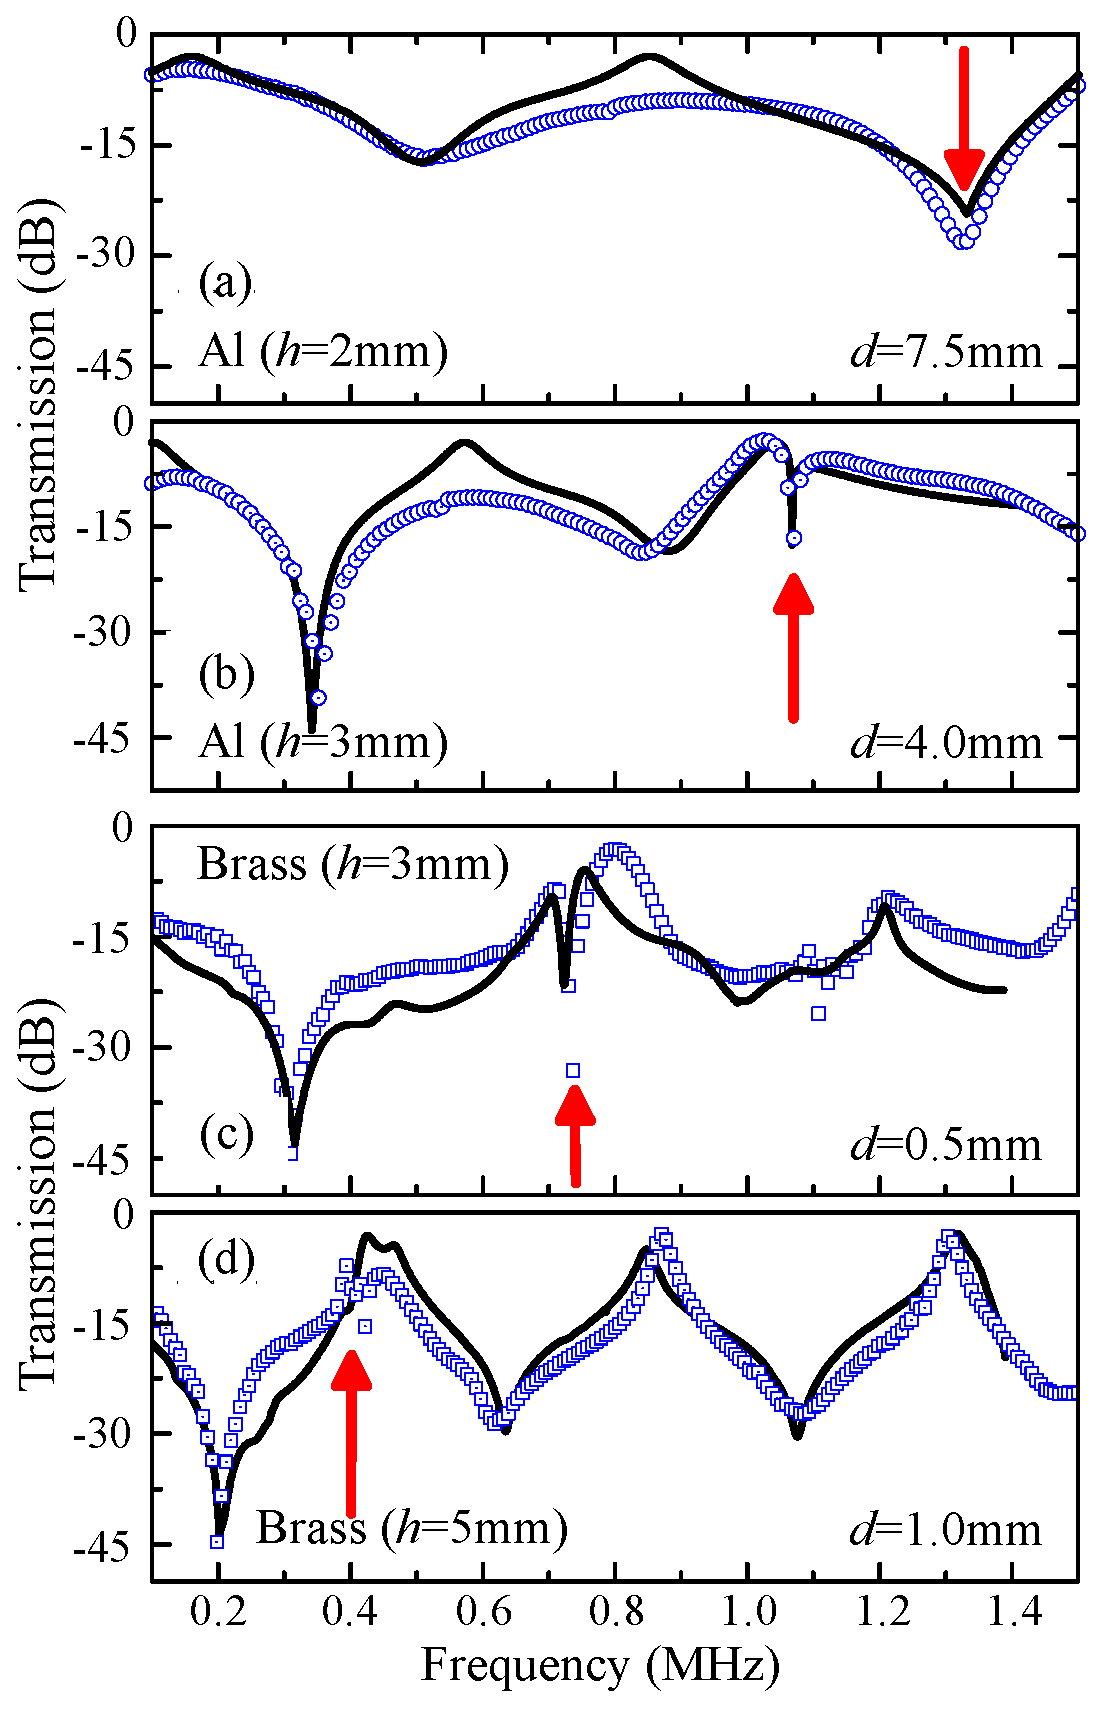
\includegraphics[width = 0.7\linewidth]{fig1_transmission_results.eps}
\caption{Sound transmission spectra of a~water slit between two aluminum (a,b) and brass (c,d) plates. Experimental results are shown by circles for aluminum and by squares for brass. Calculated spectra are shown by solid lines. The~vertical arrows mark the~minima due to the~excitation of the~slow mode.}
\label{fig:theoryexperimentRayleigh}
\end{center}
\end{figure}

\subsection{Comparison of the~Theoretical Results with the~Experiment}

In order to compare the~experimental transmission spectra \cite{channel1} with the~theoretical ones, the~transmission coefficient must be properly defined first.
The~conditions of the~experiment imply that only the~energy flux towards the~transducer surface is detected, so the~transmission coefficient should be calculated as
\begin{equation}
\label{tarn}
\mathcal{T}_{\|}(\omega) =\frac{1}{A p_0 v_{0x}} \int_A I_{x}(x=l,z) dydz
 = \frac{1}{\pi R_d^2 p_0 v_{0x}} \int_{-R_d}^{R_d} I_{x}(x=l,z) \sqrt{R_d^2-z^2} dz.
\end{equation}
Here $A=\pi R_d^2$ is the~area of the~transducer antenna, $l=8$ cm is the~$x$-coordinate of the~receiver, $p_0 v_{0x}$ is the~energy flux in the~incident wave, and 
\begin{equation}
I_{x}=p(x,z) v^{*}_x(x,z)=i \omega \rho_f T(x,z) \frac{\partial T^{\ast}(x,z)}{\partial x}
\end{equation}
is the~$x$-component of the~transmitted acoustic flux.

As shown in the~\cref{fig:theoryexperimentRayleigh}, the~theoretical spectra given by \cref{tarn} agree remarkably well with the~experimental data in a~wide frequency range for a~water ($\rho_f=1000$ kg/m$^3$, $c_f=1500$ m/s) channel.
The~fine structure of the~spectra and the~correct depth of the~minima observed at the~frequencies indicated by the~arrows are also recovered.
The~agreement is preserved when the~length and width of the~channel are varied to simulate both short and wide channels, $h < d$, \cref{fig:theoryexperimentRayleigh} (a,b), and long and narrow ones, $d < h$, \cref{fig:theoryexperimentRayleigh} (c,d), and also when the~material of the~plates is alternated between brass ($\rho_m=8400$ kg/m$^3$, $c_t=2000$ m/s, $c_l=4250$ m/s) and aluminum ($\rho_m=2700$ kg/m$^3$, $c_t=3130$ m/s, $c_l=6230$ m/s).

Indeed, as long as the~linear Hooke's law is applicable and the~viscous effects are negligible, the~calculations outlined above are guaranteed to be exact since they are based on the~exact solutions of the~wave equations.
The~stress-strain relationship is, of course, linear if the~amplitudes of the~incident wave and, consequently, of the~media vibrations are not too large.
As for the~viscous phenomena, it is known that they are manifested mainly within the~viscous layers at the~fluid-solid interfaces.
In water with the~viscosity coefficient $\nu=0.01$ cm$^2$/s these layers have a~typical thickness of approximately $\sqrt{2\mathbf{\nu}/\omega} \approx 10^{-4}$ cm in the~frequency range studied.
The~scale of the~viscous layers then appear to be several orders of magnitude smaller than the~scale of the~channel, and for that reason, the~accuracy of the~obtained results practically does not suffer if the~fluid is treated as inviscid.

The~factor that impacts the~accuracy the~most is the~number of eigenmodes that are accounted for in the~series \cref{pot1}-\cref{pot3}.
As was mentioned earlier, any propagating eigenmode that exists for a~given frequency must always be included.
On the~contrary, among the~infinite number of leaky modes choosing only the~first few in the~increasing order of their decay rates $\im\beta_n$ is sufficient.
The~actual number of leaky modes for each frequency is determined based on the~convergence of the~resulting transmission spectrum.
Naturally, the~series \cref{pot1}-\cref{pot3} converge slower for wider channels.
This is due to the~scaling $\omega_n \sim 1/d$ of the~mode eigenfrequencies.
For example, increasing the~channel width $d$ red-shifts the~cutoff frequencies \cref{eq:cutoffRayleigh} of the~propagating fast modes, so for a~wider channel a~larger number of fast modes may emerge within the~same frequency range.
In other words, the~wider the~channel the~more coupled Rayleigh modes it can support.

Specifically, the~spectra shown in \cref{fig:theoryexperimentRayleigh} (a)-(d) correspond to the~channels which support up to 8, 5, 2, and 2 propagating Rayleigh modes, respectively, in the~frequency range from 0.1 MHz to 1.4 MHz.
The~first of these modes is a~slow mode that exists for any frequency, and the~remaining fast modes start at their own cutoff frequencies \cref{eq:cutoffRayleigh}.
For the~channel of width $d=1.0$ mm between the~two brass plates, for example, the~fast mode with $n=2$ emerges at the~frequency 2.35 MHz, so obviously it cannot contribute to the~transmission below 1.4 MHz.
However, in the~twice wider channel the~same mode would appear at 1.17 MHz, and its contribution then could not be ignored.
The~number of leaky modes necessary to achieve convergence in the~cases of \cref{fig:theoryexperimentRayleigh} (a)-(d) was 11, 11, 7, and 7, respectively.
The~next leaky mode, if included in the~calculations, leads to the~variation in the~result which is considerably less than 1\%.

%The~proposed method of calculation of transmitted and reflected acoustic fields excited by a~plane wave is practically exact. The~only physical approximations we used -- the~linear Hooke's Law and inviscid fluid -- do not really affect the~accuracy of the~obtained results.  Indeed, the~width of the~viscous boundary layer $\sqrt{2 \nu/\omega} \approx 10^{-4}$ cm in water ($\nu =0.01$ cm$^2$/s) is negligible as compared with the~apertures used in our experiments. Therefore, the~calculated spectra of {\it direct} transmission
%\begin{equation}
%\label{tarn}
%\mathcal{T}_{\|}(\omega) =\frac{1}{A p_0 v_{0x}} \int_A I_{\|}(x=l,z) dydz
% = \frac{1}{\pi R_d^2 p_0 v_{0x}} \int_{-R_d}^{R_d} I_{\|}(x=l,z) \sqrt{R_d^2-z^2} dz
%\end{equation}
%are in excellent agreement with the~experimental spectra, as shown in \cref{fig:theoryexperimentRayleigh}. Here $A=\pi R_d^2$ is the~area of the~transducer antenna, $l= 8$ cm is the~coordinate of the~receiver, $p_0 v_{0x}$ is the~flux in the~incident wave, and $ I_{\|}=p(x,z) v^{*}_x(x,z)=i \omega \rho_f T(x,z) (\partial T^{\ast}(x,z)/\partial x)$ is parallel to the~channel component of the~transmitted flux of sound energy. Note that no fitting parameters were used in the~plots. The~agreement is observed within a~wide range of frequencies, for different metal plates (aluminum and brass), and for very different geometry of the~slit: short and wide channel, $h<d$, \cref{fig:theoryexperimentRayleigh} (a,b) and long and narrow channel, $d<h$, \cref{fig:theoryexperimentRayleigh} (c,d).

% The~accuracy of the~theoretical spectra depends on the~number of complex roots of \cref{disp} included in the~expansions \cref{pot}. To plot the~transmission spectra in \cref{fig:theoryexperimentRayleigh} we numerically calculated each root as a~function of frequency, i.e. each root generates a~trajectory $\xi_n(\omega)$ in the~complex $\xi$ plane (see \cref{fig:roots}).   The~convergence of the~series \cref{pot} is  slower for  wider channels, therefore in calculations of the~results shown in \cref{fig:theoryexperimentRayleigh} (a) and (b) the~number of complex roots was 11, while the~plots in \cref{fig:theoryexperimentRayleigh} (c) and (d) were obtained with only 7 complex roots.
% For all the~graphs addition of one more complex root leads to less than $1\%$ variation.
% As in any waveguide the~number of real roots (propagating modes) increases with frequency, i.e. each new real root emerges at cutoff frequency, except the~slow mode which starts from zero frequency. For the~fast mode the~cutoff frequencies $Q_n c_t/d$ are obtained from \cref{veloc}. For the~frequencies near 1.4 MHz \cref{disp} has 8, 5, 2, and 2 real roots for the~channels whose spectra are shown in \cref{fig:theoryexperimentRayleigh} (a)-(d). One of these running modes is always the~slow mode. In the~case of brass channel the~cutoff frequency for the~second ($n=1$) waveguide mode  $Q_1 c_t/d= 2.35$ MHz for the~channel with width $d=1$ mm. Therefore, it does not contribute to sound transmission in our experiments.  Its contribution becomes essential for width $d>2$ mm.

%%%%%%%%%%%%%%%%%%%%%%%%%%%%%%%%%%%%%%%%%%%%%%%%%%%%%%%%%%%%%%%%%%%%%%%%%%%%%%%%%%%%%%%%%%%%%%%%%%%%%%%%%%%%%%%%%%%%%%%%%%%%%%%%%%%%%%%%%%%%%%%%
%                                     FIGURE #3
%%%%%%%%%%%%%%%%%%%%%%%%%%%%%%%%%%%%%%%%%%%%%%%%%%%%%%%%%%%%%%%%%%%%%%%%%%%%%%%%%%%%%%%%%%%%%%%%%%%%%%%%%%%%%%%%%%%%%%%%%%%%%%%%%%%%%%%%%%%%%%%%%%%%%%%
\begin{figure}
\begin{center}
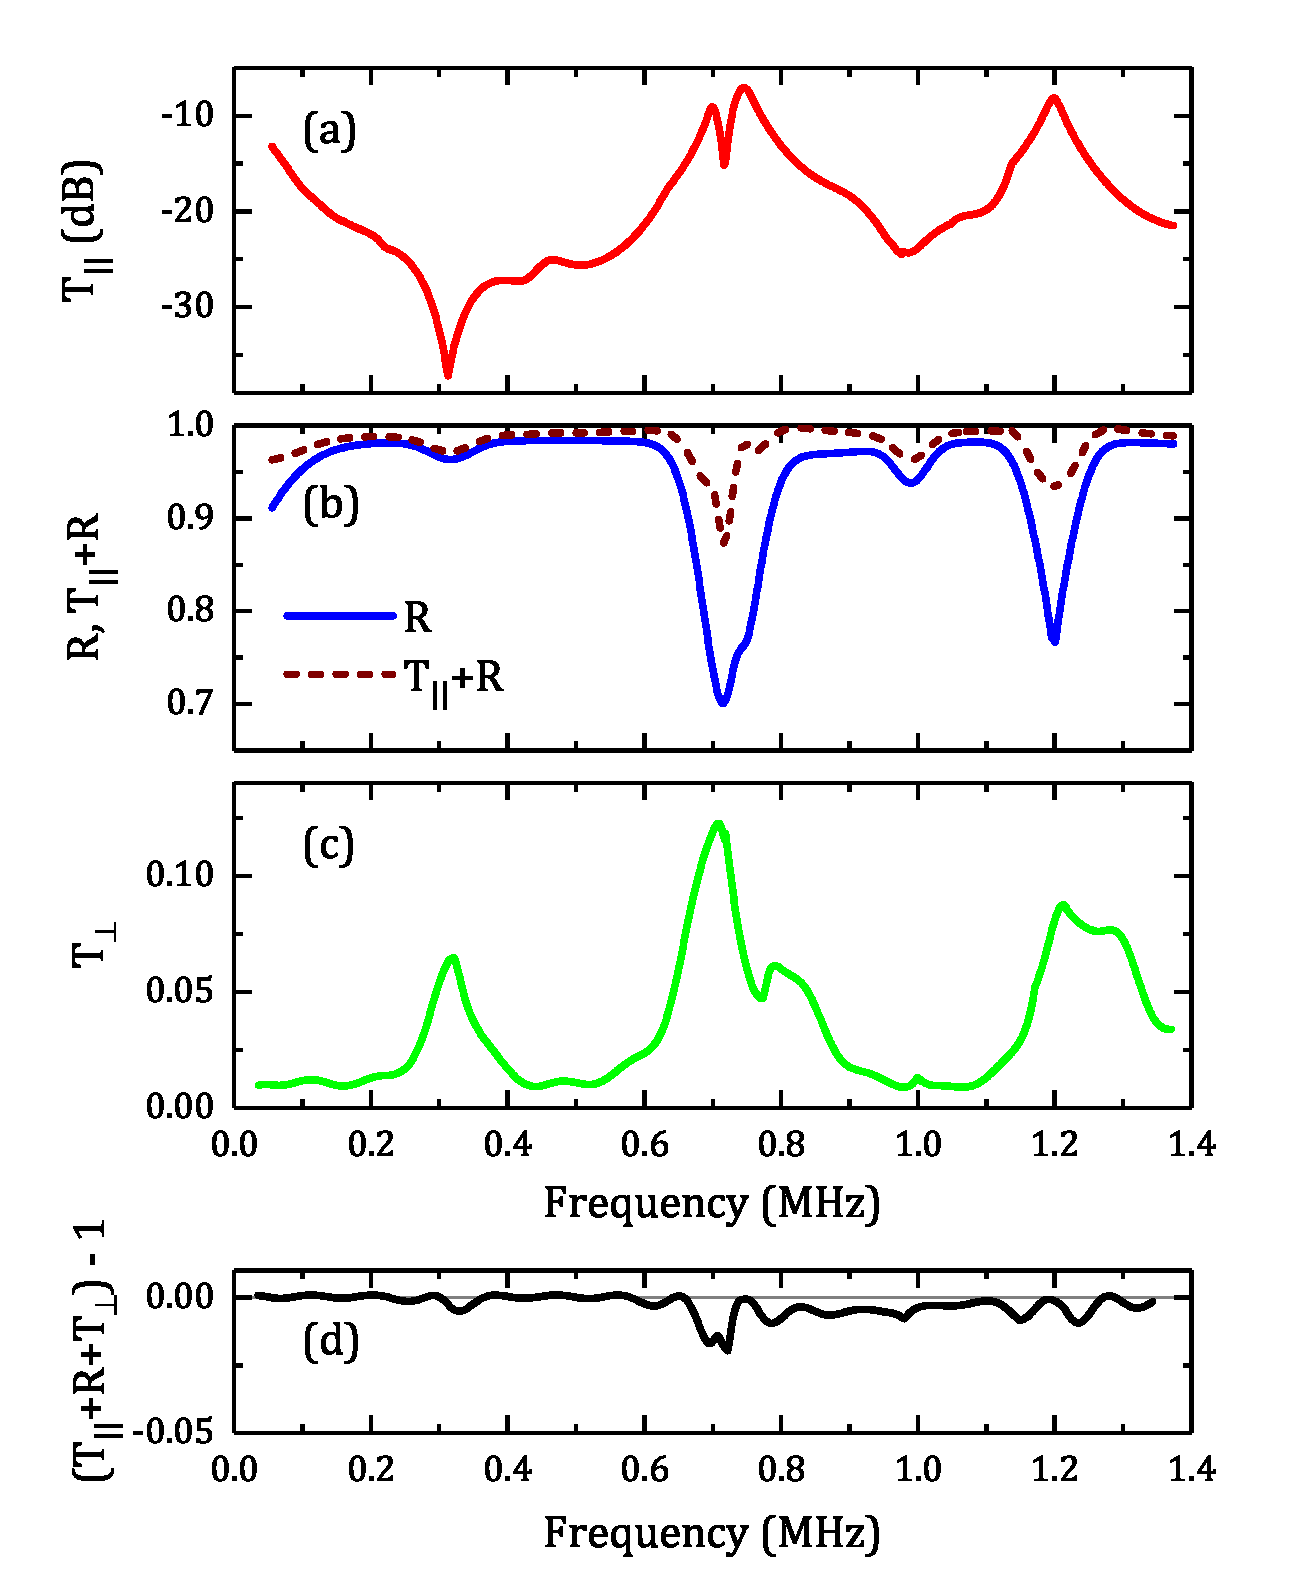
\includegraphics[width = 0.8\linewidth]{TrRe.eps}
\caption{Calculated transmission and reflection spectra for two brass plates with sides of length $L=12$ cm separated by a~channel with $h =3$ mm and $d=0.5$ mm.  (a) Transmission through the~solid vertical boundary $x = h$ (solid red line) in log scale. (b) Reflection from the~solid vertical boundary $x=0$ (blue), and the~sum $T_{\|}+R$ (brown dashed line). (c) Transmission through the~horizontal boundary $z = d/2$. (d) The~conservation of energy as demonstrated by the~sum $T_{\|}+T_{\perp}+R$, which does not deviate from 1 by more than $2\%$.}
\label{fig:fig3}
\end{center}
\end{figure}

\subsection{Redirection of Sound into Elastic Plates}

Additional insights into the~physical reasons for the~extraordinary low transmission in \cref{fig:theoryexperimentRayleigh} can be gained by the~examination of how the~acoustic energy is scattered in the~system.
For the~water channel with $h=3$ mm and $d=0.5$ mm with the~spectrum shown in \cref{fig:theoryexperimentRayleigh}(c) I calculate both the~transmission and the~reflection spectra.
These two coefficients are redefined here in order to account for the~total flux in the~$x$-direction through the~entire solid boundaries $x=0$ and $x=h$:
\begin{equation}
T_{\|} = 2\frac{i \omega \rho_f^2 c_f }{p_0^2 L} \int_{d/2}^{\infty} T(h,z)\left.\frac{\partial T^{*}(x,z)}{\partial x}\right|_{x=h}\, dz,
\end{equation}
\begin{equation}
R = -2\frac{i \omega \rho_f^2 c_f }{p_0^2 L} \int_{d/2}^{\infty} R(0,z)\left.\frac{\partial R^{*}(x,z)}{\partial x}\right|_{x=0}\, dz.
\end{equation}
Also, I calculate the~flux that is transmitted from the~water channel into the~plates through the~boundaries $z=\pm d/2$:
\begin{equation}
T_{\perp} = 2\frac{i \omega \rho_f^2 c_f }{p_0^2 L} \int_{0}^{h} B(x,z)\left.\left(\frac{\partial B^{*}(x,z)}{\partial z}\right)\right|_{z=\frac{d}{2}}\, dx.
\end{equation}

The~three curves are shown in \cref{fig:fig3}.
Interestingly, at the~frequencies where the~minima in transmission are observed the~reflection is also suppressed (see \cref{fig:fig3} (b)).
Calculation of the~sum of the~fluxes exiting from either vertical side of the~plate reveals that there must be an~additional energy supplied to the~plates as the~sum $T_{\|}+R$ falls considerably below 1 for a~wide range of frequencies.
Clearly, this additional portion of energy has to be coming from the~fluid channel through the~channel walls.
The~spectrum of this vertical flux, $T_{\perp}$, is shown in \cref{fig:fig3} (c).
The~minima of $T_{\|}$ and $R$ coincide with the~maxima of $T_{\perp}$, and the~total flux that goes through the~sides of the~plates is very close to 1 which is expected as the~total energy must be conserved in the~system (see \cref{fig:fig3} (d)).
The~flux through the~other end of the~plate, at $z=\infty$, is negligible as all of the~leaky Rayleigh modes carrying energy will necessarily be scattered through the~vertical sides in a~sufficiently long plate.
The~minor fluctuations of $T_{\|}+R+T_{\perp}$ around 1 are due to the~numerical error that builds up during the~calculations.
The~analysis performed here stresses that the~channel system cannot be regarded as an~aligned along $z$-axis 1D scatterer of acoustic waves.

The~elastic nature of plates in the~2D system studied allows for an~interesting ability to redirect the~acoustic excitation into the~plates.
The~waves in the~plates may then propagate perpendicular to the~direction of the~incident wave.
This feature can not be described in the~models employing the~rigid-body approximation which is quite commonly used in a~great number of acoustic studies.
Therefore, only the~elastic screens have the~capability to redirect sound into metal at an~almost $90^o$ angle.
The~redirected flux can be observed to be as high as 12\%, as can be seen from \cref{fig:fig3} (c) for the~frequency of around 0.7 MHz.
This is quite a~strong effect, and the~amount of redirected flux can be comparable with the~flux transmitted through a~brass plate in water (as low as 8\%, or $-11$ dB, for the~frequency of the~Fabry-Perot minimum).

%In order to analyze physical nature of the~deep minima in \cref{fig:theoryexperimentRayleigh}, we calculated the~reflection spectrum for the~slit with $h=3$mm and $d=0.5$ mm and plotted it in \cref{fig:fig3} together with the~total transmission $T_{\|}$ through the~whole boundary $x=h$.

%The~positions of the~minima in the~reflection in \cref{fig:fig3} (a) coincides with the~positions of the~minima in the~transmission in \cref{fig:theoryexperimentRayleigh} (c).  Near these minima the~sum of forward and backward scattered flux, $T_{\|}+R$, is considerably less than 1, that is a~clear indication that this sum does not represent the~total flux scattered by the~slit. Since the~slit shown in \cref{fig:theoryexperimentRayleigh} is a~2D scattering system,  the~lack of scattered flux, $1-T_{\|}-R$, is the~energy scattered along axis $z$.
%In \cref{fig:fig3}b we plot the~spectrum transmitted from the~fluid to the~metal through the~horizontal boundary $z=d/2$.
%It exhibits maxima exactly at the~frequencies where $T_{\|}+R$ exhibits minima, thus representing the~flux, $T_{\perp}$, which is lost if the~slit is approximated as a~1D scatterer.
%The~total scattered flux $T_{\|}+T_{\perp}+R$, while fluctuates due to numerical errors, still remains very close to 1, as it is shown in the~inset to \cref{fig:fig3}b.

%Vibrations of the~metal-fluid boundary $z=\pm d/2$ break 1D symmetry of the~system, {\bf i.e. these boundaries are not flat any more.  This broken symmetry} gives rise to the~elastic wave propagating in the~metal plates perpendicular to the~incident wave.  The~flux of energy $T_{\perp}$ associated with this redirected wave does not appear in the~model of rigid screen which was accepted in many previous studies. Therefore, the~property of a~slit to redirect the~incoming flux into metal is manifested only for elastic screens. The~amount of redirected acoustic energy may reach $12\%$ at the~frequencies near 0.7 MHz, as shown in \cref{fig:fig3}. This is relatively strong effect, taking into account that a~brass plate in water transmits only about $8\%$ (-11 Db) in the~minimum of the~Fabry-Perot resonance. 

%%%%%%%%%%%%%%%%%%%%%%%%%%%%%%%%%%%%%%%%%%%%%%%%%%%%%%%%%%%%%%%%%%%%%%%%%%%%%%%%%%%%%%%%%%%%%%%%%%%%%%%%%%%%%%%%%%%%%%%%%%%%%%%%%%%%%%%%%%%%%%%%%%%%%%%%%%%%%
%                                                               FIGURE #4
%%%%%%%%%%%%%%%%%%%%%%%%%%%%%%%%%%%%%%%%%%%%%%%%%%%%%%%%%%%%%%%%%%%%%%%%%%%%%%%%%%%%%%%%%%%%%%%%%%%%%%%%%%%%%%%%%%%%%%%%%%%%%%%%%%%%%%%%%%%%%%%%%%%%%%%%%%%%%
%
\begin{figure}
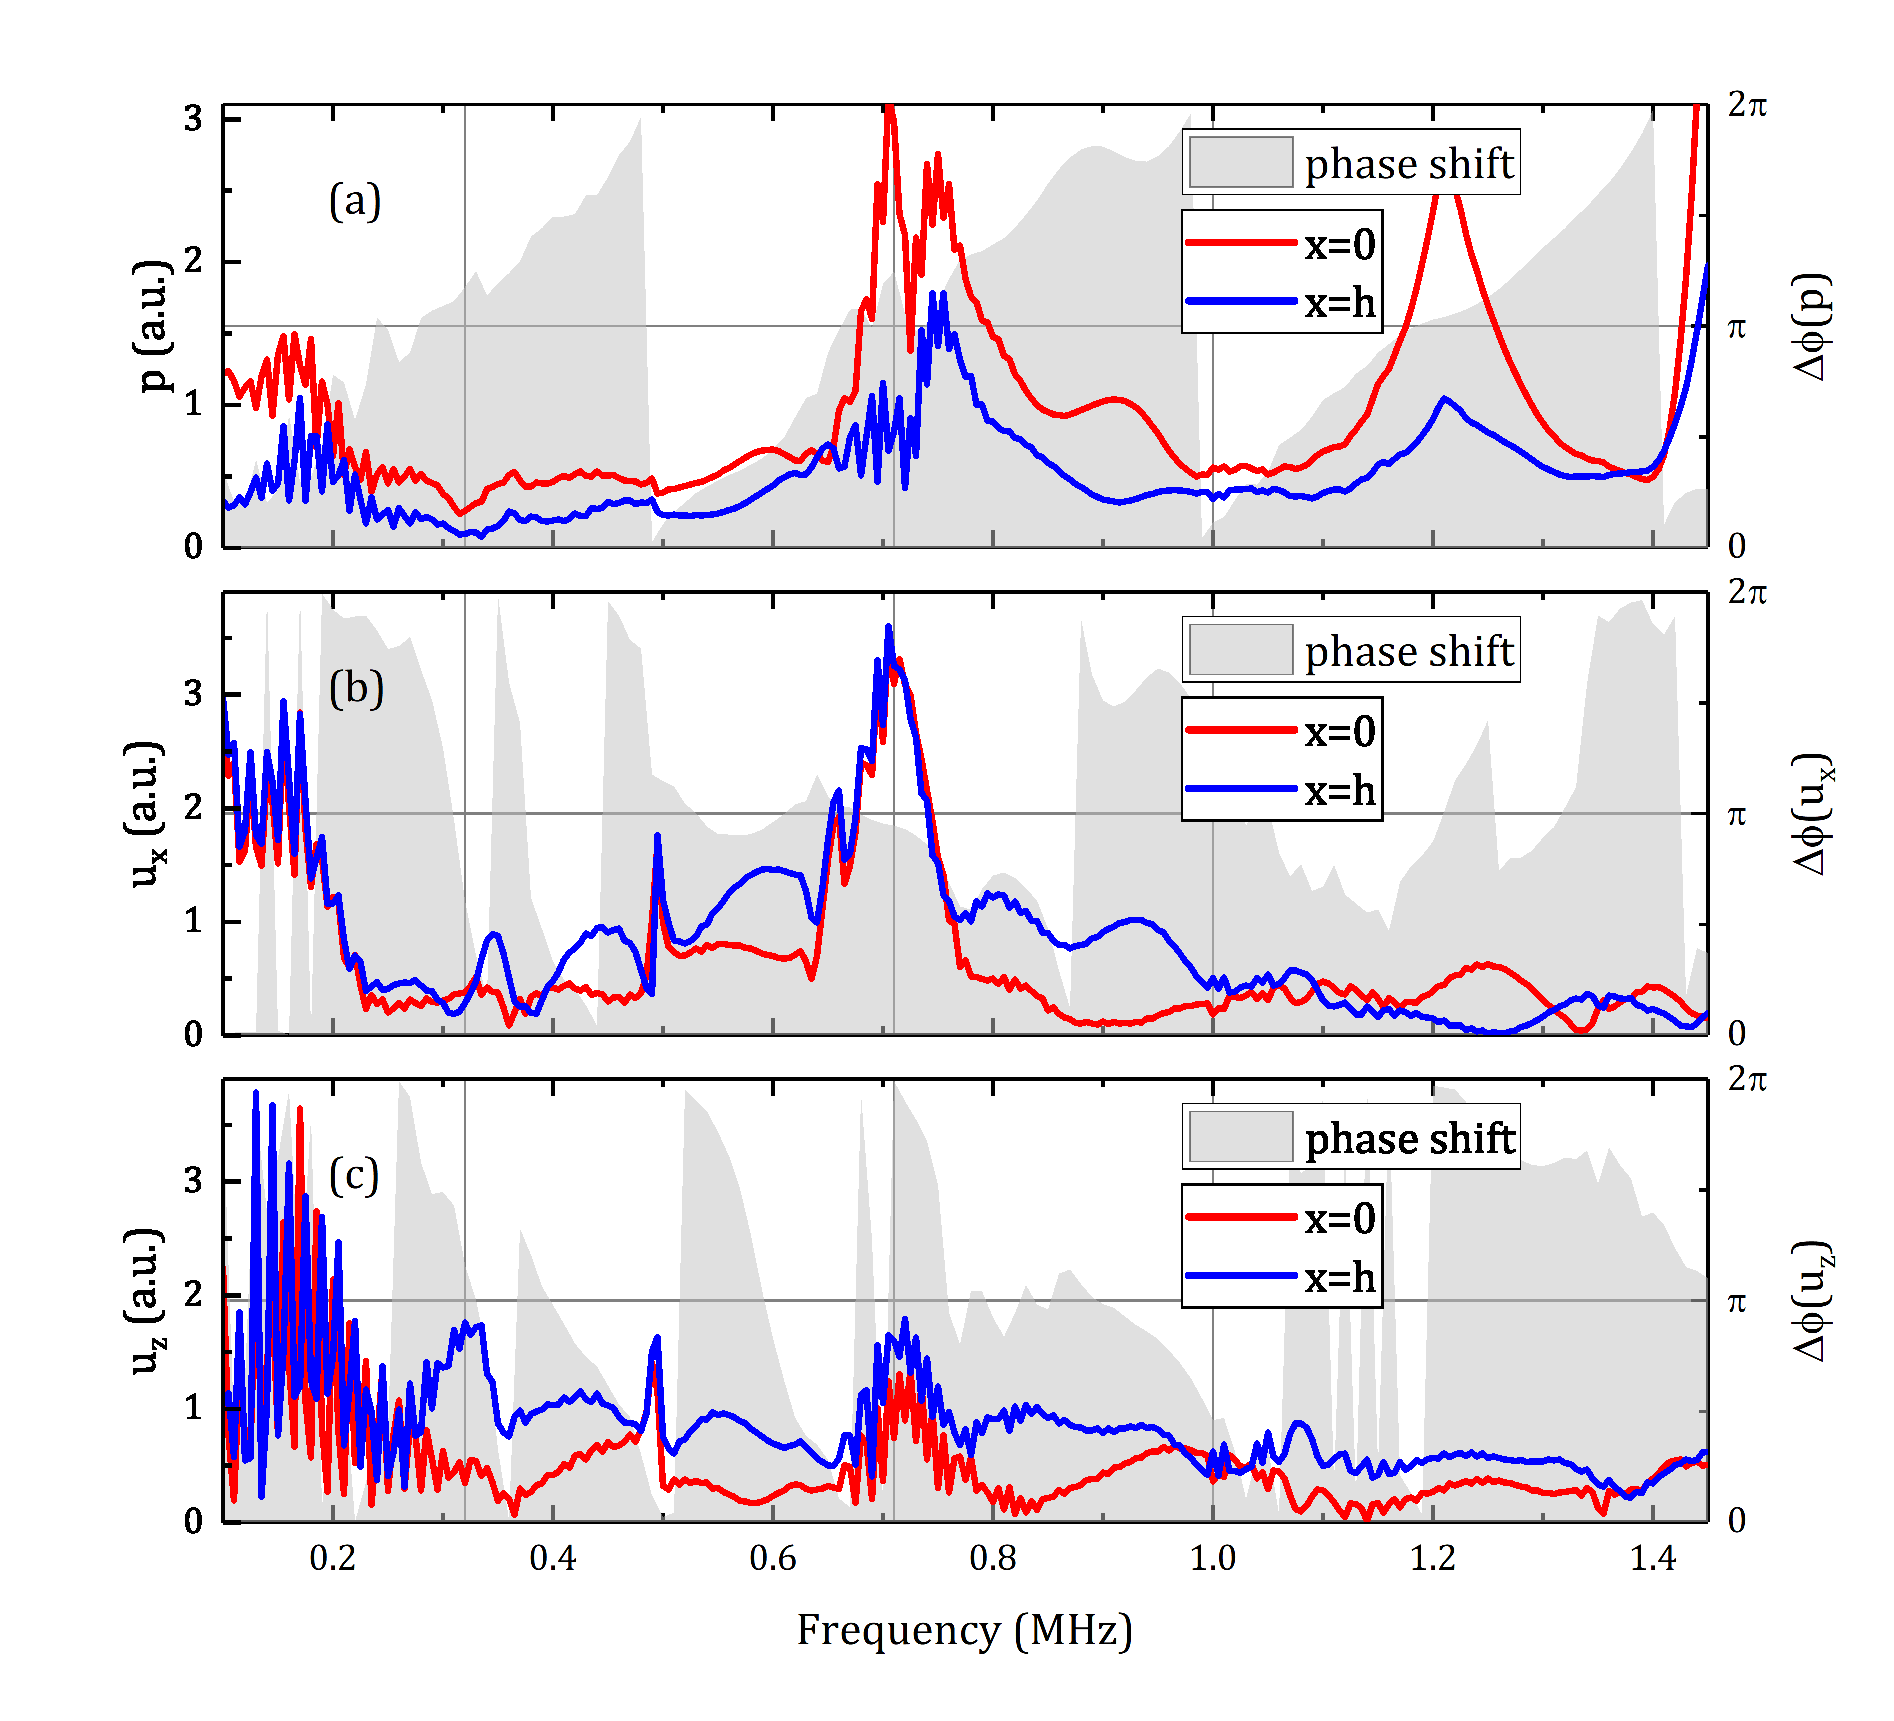
\includegraphics[width=0.9\linewidth]{p_ux_uz.eps}
\caption{Frequency dependence of the~pressure, $x$ and $z$ displacement of the~plates at the~left and right ends of the~same channel as in \cref{fig:fig3}. The~solid curves show the~amplitude of the~respective quantity calculated at the~points $x=0$ (red) and $x=h$ (blue). The~shaded regions represent the~phase shifts $\Delta\phi(g)=\arg \left.g\right|_{x=0}-\arg \left.g\right|_{x=h}$ for each quantity $g=p,u_x,u_z$ whose amplitudes are plotted in the~same panel. Straight vertical lines mark the~positions of the~deep minima in the~transmission shown in \cref{fig:theoryexperimentRayleigh} (c).}
\label{fig:fig4}
\end{figure}


In order to understand how individual Rayleigh eigenmodes enhance the~radiation of energy into the~plates, I analyze frequency dependence of the~pressure and both $x$- and $z$-components of the~displacement vector evaluated at the~corners of the~channel ($x=0,h$, and $z=d/2$).
The~respective graphs are visualized in \cref{fig:fig4}.
Each panel of the~figure is dedicated to a~certain physical quantity.
The~solid lines show the~amplitudes of that quantity for either corner of the~channel as a~function of frequency, and the~shaded area gives the~relative phase shift between the~two.

For the~resonant frequencies that correspond to the~minima in transmission (0.32 MHz, 0.71 MHz, and 0.98 MHz) the~horizontal displacement appears to have very small amplitudes close to the~first and third resonances (which are basically the~Fabry-Perot minima).
In the~second resonance the~amplitudes are quite large, and the~phase shift is close to $\pi$, meaning the~vibrations are out of phase.
This corresponds to high transmission of sound, so the~appearance of the~dip must be caused by another factor.
Namely, the~pressure at both ends of the~channel in the~resonances is close to zero or exhibits a~sharp dip.
As for the~vertical displacement, its contribution to the~redirection of sound is due either to the~amplitudes at each corner being close and in phase (close to $0$ or $2\pi$), or one amplitude being much larger than the~other.

Both the~suppressed direct transmission and the~suppressed reflection are necessary conditions to have the~strong redirection of flux into the~metal plates.
This requires having simultaneously low pressure $p(x,z)$ and small amplitudes of horizontal vibrations $u_x(x,z)$ of the~plate boundaries at the~channel ends.
Naturally, when the~pressure minima occur at the~same (or very close) frequencies as the~displacement minima, the~extraordinary low transmission of sound ensues.
The~sharpness of the~dip in \cref{fig:theoryexperimentRayleigh} correlates with the~amount of energy being redirected.
The~closer the~frequencies for which both $p$ and $u_x$ are low, and the~closer these quantities are to zero, the~sharper becomes the~dip, and, consequently, the~more energy veers into the~metal.
Moreover, it helps to have the~local maxima for the~$z$-component of the~displacement at the~resonant frequency to facilitate the~redirection of energy into the~metal.
While the~frequency dependence on every individual panel in \cref{fig:fig4} exhibits the~described behavior for multiple frequencies, the~effect builds up when this behavior is manifested simultaneously, i.e., at the~same frequency.
For example, the~third resonance is much broader than the~other due to quite weak vertical oscillations of the~plate boundaries.

Qualitatively, one can conclude about the~strength of the~effect based on how different eigenmodes propagating in opposite directions in the~channel interfere to form standing (or, better to say, quasi-standing) waves across the~length of the~channel $h$.
Indeed, since the~propagating Rayleigh eigenmodes exhibit usual oscillating behavior along the~$x$-axis, the~low pressure at the~channel ends occurs when the~modes interfere destructively.
Specifically, the~most suppression of transmission results from the~destructive interference of the~eigenmode which would otherwise contribute the~most to the~transmission.
If at the~same frequency another eigenmode interferes destructively as well, the~dip in the~spectrum becomes even sharper.
Even though it is possible to conclude how the~modes interfere, it is, nevertheless, quite challenging to determine how much energy is redirected as a~function of the~channel geometry since it explicitly depends on the~dispersion \cref{eq:dispersionXiRayleigh} of each involved Rayleigh eigenmode.

The~two principal maxima in transmission, at 0.71 MHz and 1.22 MHz, are the~maxima of the~Fabry-Perot resonances, and they simply coincide with the~minima in the~reflection spectrum.
Also, the~amplitude of the~transmitted pressure is quite large (see \cref{fig:fig4}(a)).
Since these Fabry-Perot maxima result from the~constructive interference of the~quasi-longitudinal leaky Rayleigh mode, their positions are strongly affected by the~mode dispersion.
The~Fabry-Perot resonances of the~bulk metal plate are equidistant in the~frequency spectrum, where as for the~system with the~channel the~maxima get closer to each other for higher frequencies.
This is due to the~phase speed of the~quasi-longitudinal mode decreasing with frequency, as shown in \cref{fig:roots}.

In \cref{fig:theoryexperimentRayleigh}(c) the~two minima in transmission at 0.32 MHz and 0.71 MHz in transmission arise due to the~constructive interference of the~propagating eigenmodes with the~phase speeds $\xi_1 = 0.99$ and $\xi_2 = 0.715$, respectively.
The~mode responsible for the~minimum at 0.32 MHz is a~fast mode that could be excited only above its cutoff frequency of about 0.3 MHz.
Its phase velocity is greater than the~speed of sound in water, $c=c_t\xi_1 > c_f$.
This minimum coincides with the~Fabry-Perot maximum, thus producing an~asymmetric fine structure in the~transmission spectrum.

The~second minimum is created by a~slow mode, which propagates slower than the~pressure wave in water.
Both minima caused by the~respective eigenmodes are quite sharp due to the~suppression of the~principal mode that is responsible of transmitting the~most energy through the~channel.


%\subsection{Verification by FEM Modeling}
The~results described above were independently verified by simulating the~transmission of sound using the~finite element method (FEM) \cite{channel2}. %with the~COMSOL Multiphysics\textsuperscript{\textregistered} software .
The~simulated spectra provided the~agreement with both the~theory and the~experiment and illustrated how the~elastic waves initially localized near the~channel walls are transformed into the~leaky waves as they propagate in the~channel.
The~viscous effects were omitted in the~simulations, which confirmed that the~observed transmission features are not due to the~unaccounted dissipation in water.

%\textcolor{red}{add here}

%The~first root corresponds to excitation of the~ fast mode, since its phase velocity $c_t \xi_1$ exceeds the~speed of sound in the~fluid $c_f$. For the~second root, $\xi_2$, the~phase velocity of the~corresponding eigenmode is less than $c_f$, therefore this minimum is due to excitation of the~slow mode.
%The~minima associated with excitation of the~slow mode are marked by arrows in the~transmission spectra shown in \cref{fig:theoryexperimentRayleigh}.
%As a~rule, these minima are sharp and asymmetric, except the~minimum at 0.4 MHz in \cref{fig:theoryexperimentRayleigh} (d), which structure is strongly affected by a~standard Fabry-Perot resonance.

%Enhanced radiation of sound into metal occurs due to large amplitude of vertical vibrations $u_z$ of the~plate boundaries at $z= \pm d/2$. Suppressed direct transmission and reflection originate from low pressure $p(x,z)$ at the~channel ends and also from small amplitude of horizontal vibrations $u_x$ of the~plate boundaries $x= 0$ and $x=h$. When these two effects occur at close frequencies they mutually enhance each other, leading to extraordinary low transmission. {\bf The~sharper a~dip in \cref{fig:theoryexperimentRayleigh}, the~more energy is redirected into metal. The~sharpness of a~dip depends on how close to zero the~pressure $p(x,z)$ and the~displacement $u_x$ become at $x= 0,h$. Being represented by  a~sum of plane waves taken over the~roots of the~dispersion equation, these quantities become small when those plane waves that give the~principal contribution interfere almost destructively at the~length of the~channel $h$. It may accidentally occur that two plane waves with \textit{smaller} amplitudes also interfere destructively, thus leading to even sharper dip. It is, however, \textit{nearly} impossible to predict how the~amount of redirected energy depends on the~geometry of the~channel and frequency, since it depends on the~values of real roots of the~transcendental equation \cref{disp}.


%In \cref{fig:fig4} we plot the~pressure and the~ amplitudes of horizontal and vertical vibrations at the~channel ends ($x = 0,h$) vs frequency. It is clearly seen that near the~resonant frequencies where minima in the~transmission are experimentally observed (marked by vertical lines) the~amplitude of horizontal vibrations of the~both faces of the~plates is close to zero.  The~same is true for the~pressure at the~ends of the~channel. Since the~vibrations of the~plates and the~fluid are coupled through the~boundary conditions, we conclude that a~quasi-standing wave is formed in the~whole system due to interference between two eigenmodes propagating in opposite directions.
%At the~same resonant frequencies the~amplitude of the~vertical vibrations reaches its local maxima that explains strong radiation into metal. While the~graphs in \cref{fig:fig4} exhibit many peaks, strong redirection of sound occurs when minimum in pressure and displacement $u_x$ coincides with maximum in displacement $u_z$. The~depth and width of the~minimum in $T_{\|}$ depends on how close to each other these three extrema occur. For example, the~first two minima at 0.32 and 0.71 MHz in Figs. \cref{fig:theoryexperimentRayleigh} (c) and \cref{fig:fig3} (a) are well pronounced since the~frequencies of all three extrema practically coincide. Unlike this, the~third minimum at 1 MHz is quite broad due to visible shifts in the~positions of the~extrema.
%There are two Fabry-Perot resonances at 0.72 and 1.22 MHz in the~transmission spectrum in \cref{fig:theoryexperimentRayleigh} (c). Here the~situation is quite simple and standard --  maximum in transmission coincides with minimum in reflection.
%This also can be seen from \cref{fig:fig4} (b) where the~amplitude of longitudinal vibrations at the~right face ($x=h$) of the~plate exceeds that on the~left face ($x=0$), especially for the~resonance at 1.22 MHz which is not affected by close proximity of a~deep minimum in transmission. 

%In \cref{fig:theoryexperimentRayleigh} (c) two minima at 0.32 and 0.71 MHz in transmission are associated with appearance of the~real roots of \cref{disp}, $\xi_1 = 0.99$ and $\xi_2 = 0.715$, respectively. The~first root corresponds to excitation of the~ fast mode, since its phase velocity $c_t \xi_1$ exceeds the~speed of sound in the~fluid $c_f$. For the~second root, $\xi_2$, the~phase velocity of the~corresponding eigenmode is less than $c_f$, therefore this minimum is due to excitation of the~slow mode.
%The~minima associated with excitation of the~slow mode are marked by arrows in the~transmission spectra shown in \cref{fig:theoryexperimentRayleigh}.
%As a~rule, these minima are sharp and asymmetric, except the~minimum at 0.4 MHz in \cref{fig:theoryexperimentRayleigh} (d), which structure is strongly affected by a~standard Fabry-Perot resonance.





%++++++++++++++++++++++++++++++++++++++++++++++++++++
%\section{FEM Numerical Modeling}
%++++++++++++++++++++++++++++++++++++++++++++++++++++

%\begin{figure}
%\begin{center}
%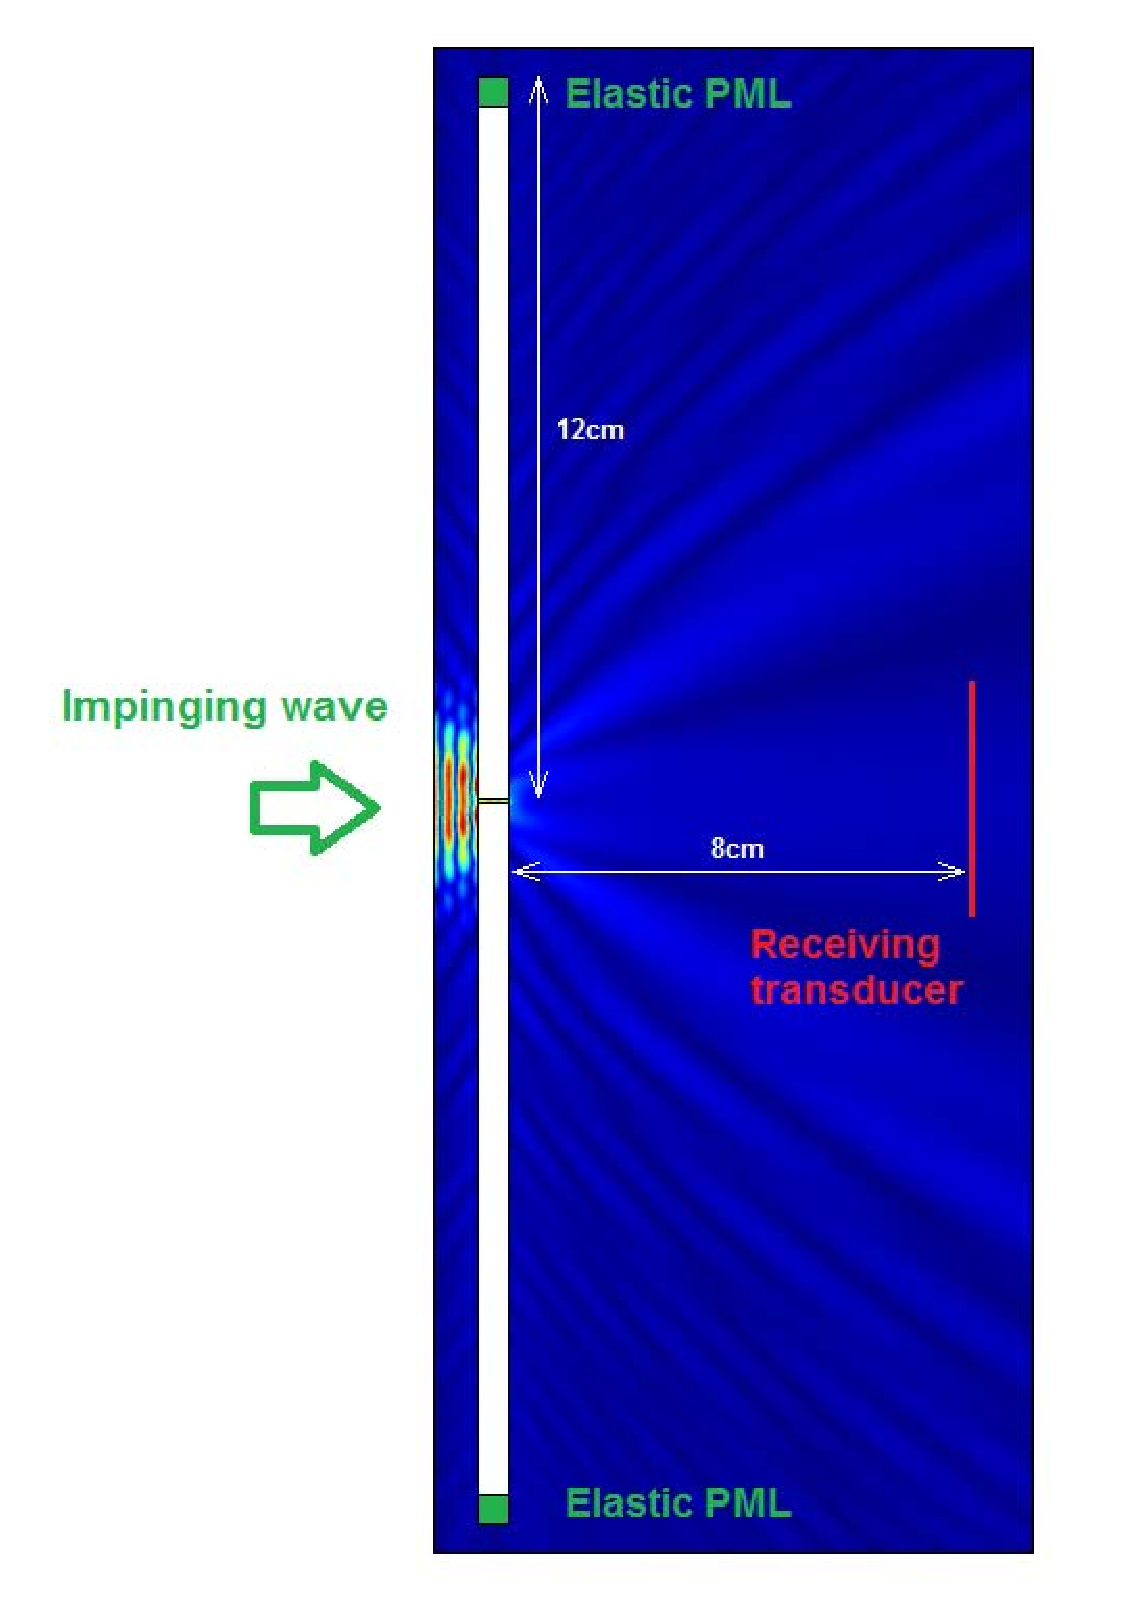
\includegraphics[width = 0.5\linewidth]{figS1.eps}
%\caption{ The~structure of the~fluid channel used for numerical simulations. A~Gaussian beam coming from the~left is incident on the~channel and the~pressure field is calculated behind the~plates. The~illustrated pattern corresponds to two brass plates with $h=5$ mm, $d=1$ mm at the~frequency 0.32 MHz.}
%\label{fig:fig5}
%\end{center}
%\end{figure}

%\begin{figure}
%\begin{center}
%\includegraphics[width = \linewidth]{figS2.eps}
%\caption{ Transmitted pressure at the~receiving antenna (in dB) for a~slit between two brass plates with $h=3$ mm (top) and $h=5$ mm (bottom) at several apertures and frequencies. Left (right) panels correspond to experimental (simulated) data.}
%\label{fig:fig6}
%\end{center}
%\end{figure}
%
%The~obtained results are additionally verified by simulating the~transmission of sound using the~finite element method (FEM).
%The~simulation was performed using the~COMSOL Multiphysics\textsuperscript{\textregistered} software, and the~geometry is shown in \cref{fig:fig5}.
%In the~model, the~two elastic plates of thickness $h$ were placed inside the~2D inviscid water domain at a~distance $d$ from each other.
%To closely match the~conditions of the~experiment, the~plates were modeled having the~same length $L=12$ cm in the~$z$ direction.
%\textcolor{red}{PMLs???}
%The~acoustic wave generated by the~transducer on the~left was approximated by a~Gaussian beam of similar effective cross section.
%The~water domain is modeled as infinite one, which is realized by imposing non-reflecting boundary conditions on the~domain's limiting borders.
%The~transmission is calculated by integrating the~sound intensity over the~vertical line of length $2R_d$ at a~distance $l=8$ cm from the~plates, which imitates the~surface of the~receiving transducer.
%The~transducer itself is not physically present in the~model.
%
%The~transmission spectra were calculated in the~frequency range from 0 to 1 MHz, with an~additional parameter sweep for the~channel width $d$ from 0 to 7.5 mm.
%The~parameters of brass were used for the~elastic properties of the~plates, and their thickness was either 3 or 5 mm.
%The~resulting data is represented by color maps in \cref{fig:fig6} on the~right panels, where the~transmission is plotted as a~function of frequency and channel aperture.
%The~left panels show the~experimental measurements, which were performed by an~automated setup for the~same parameter ranges.
%
%\textcolor{red}{change below}
%Theoretical and experimental results are also supported by finite element simulations, which were performed through the~commercially available software COMSOL Multiphysics. The~employed model is represented in \cref{fig:fig5}. It consists of a~two-dimensional domain filled with a~fluid having the~acoustic properties of water. Two elastic plates with thickness $h$ and separated by a~distance $d$ are displaced forming a
%fluid channel. The~plates are of the~same length of 12 cm as the~experimental samples.  At the~ends the~both plates terminate with two additional absorbing domains (or elastic perfectly matched layers, PML) in order to suppress reflection. Normally incident Gaussian beam is used as impinging wave to provide a~more realistic excitation. The~exterior boundaries of the~model are configured with non-reflecting conditions, ensuring that outgoing waves leave the~domain.

%A~frequency sweep is performed numerically for different thicknesses $h$ and apertures $d$ of the~slit. This process provides a~large amount of data which can be summarized through maps showing the~transmitted pressure as a~function of frequency and aperture. In addition, the~same sweep was also experimentally carried out using an~automated setup. In \cref{fig:fig6} we compare experimental and numerical data for brass plates with thickness $h=3$ mm and $h=5$ mm.
%The~numerical data are obtained by integrating the~pressure field over the~length of the~receiving transducer (see \cref{fig:fig5}).

%Both maps exhibit regions of parameters with anomalously low transmission. There is excellent agreement between the~positions of the~deep minima obtained experimentally, theoretically, and numerically. The~deepest minima  at 0.32 MHz for $h=3$ mm and at 0.2 and 0.64 MHz for $h=5$ mm appear as bright blue spots in the~maps in \cref{fig:fig6}.
%Unlike this, less deeper minima at 0.71 MHz ($h = 3$ mm) and at 0.4 MHz ($h=5$ mm) appear as narrow yellow lines on red background. This occurs because these local minima are close to the~maxima of the~Fabry-Perot resonances. These less-deeper minima correspond, as it is explained in the~main text, to excitation of the~slow mode. The~minimum at 0.4 MHz ($h=5$ mm) has a~doublet structure (see \cref{fig:theoryexperimentRayleigh}d), which is well-reproduced in the~experimental map in \cref{fig:fig6}.
%It, however, is not resolved in our numerical simulations.
%It is worth mentioning that no viscosity effects were considered in the~fluid, thus demonstrating that the~reported effects are not due to viscous phenomena inside the~channel.
%
%The~elastic displacements were also obtained from the~simulations, allowing the~observation of the~wave phenomena occurring inside the~plates.
%A~motion picture showing the~pressure map in the~fluid superimposed with the~lines of displacement (either in water or metal) is presented in the~Supplementary Material Movie S1 \cite{supp}.
%It is calculated for brass plates with $h=3$mm and $d=0.5$mm (the~same parameters as in \cref{fig:theoryexperimentRayleigh}c) at 0.704 MHz.
%It is shown how the~incoming wave generates elastic vibrations inside the~slit and the~plates and how these vibrations propagate. It is easy to see that that the~vibrations of the~plate which originally are localized near the~channel boundaries become leaky modes, carrying the~acoustic energy away from the~channel in a~form of vortices. The~vortex structure of the~displacement field in metal is due to non-potential contribution $\nabla \times S$ to the~displacement field $\bf u$. This  movie visualizes the~effect of redirection of sound by a~straight fluid channel with elastic boundaries.



%%%%%%%%%%%%%%%%%%%%%%%%%%%%%%%%%%%%%%%%%%%%%%%%%%%%%%%%%%%%%%%%%%%%
\section{Summary}
A~comprehensive study of sound transmission through a~fluid channel surrounded by elastic regions is presented in this chapter.
The~rigorous analytical solution of the~scattering problem allows to calculate the~transmission spectrum that almost coincides with the~experimental transmission data.
It is theoretically discovered that the~system exhibits an~unusual behavior --- the~behavior of a~redirecting acoustic antenna.
The~ability of the~fluid channel to redirect the~acoustic energy at an~almost $90^o$ angle into the~surrounding elastic media is quite strong, allowing to affect up to approximately 10\% of the~incoming flux.
The~phenomenon discussed above was previously unknown for the~fluid channels, and it is explained in terms of the~mutually interfering coupled Rayleigh eigenmodes of the~channel.
Simply put, whenever the~vibrations of the~fluid and the~elastic media become synchronized and form one or several quasi-standing waves in the~system, the~transmission forward and the~reflection backward are suppressed and the~acoustic flux escapes in the~remaining unusual direction.

The~analytical approach developed for this problem employs the~method of expanding the~acoustic fields over the~set of eigenmodes of the~system.
The~lack of orthogonality of the~eigenmodes does not allow for the~completely analytical solution, nevertheless, the~obtained numerical solution is  practically exact.
This approach can be applied to other problems with more complicated geometries, such as elastic screens with periodically arranged apertures.

The~effect of the~redirection of sound is important for designing of the~acoustic devices that are able to manipulate the~propagation of sound, such as acoustic waveguides or acoustic antennas.

%In summary, we reported a~comprehensive study of sound transmission through a~finite-length fluid channel with elastic boundaries. It is experimentally observed and explained and how a~straight fluid slit between two metallic screens may serve as a~redirecting acoustic antenna.
%This previously unknown property is due to excitation and interference of the~eigenmodes which describe the~synchronized vibrations of the~fluid and metal plates.
%Maximum of energy redirected into the~plates occurs when \textbf{as many eigenmodes as possible become quasi-standing waves on the~length of the~channel simultaneously}.
%The~proposed method of solution of the~scattering problem for a~slit is practically exact and leads to excellent agreement with the~experiment. The~proposed analytical approach may be easily extended to more complicated geometries, in particular, to a~set of periodically arranged slits.
%The~effect of redirection of sound may find applications in design of specific devices for  manipulation of acoustic energy and vibration of plates embedded into fluids. The~resonant modes which are responsible for the~redirection of sound are of particular interest for microfluidics since pressure produced by the~vibrating boundaries is comparable with the~capillarity force or the~force generated by a~micropump.






%%% Local Variables: 
%%% mode: latex
%%% TeX-master: "dissertation"
%%% End: 
